\documentclass{article}
\usepackage{xeCJK}
\usepackage{amsmath}
\usepackage{amssymb}
\usepackage{mathrsfs}
\usepackage{xcolor}
\usepackage{bm}
\usepackage{hyperref}
\usepackage{graphicx}
\usepackage{subcaption}
\usepackage{float}
\usepackage{multicol}
\usepackage{pdfpages}
\usepackage{csquotes}
\usepackage[ruled,linesnumbered]{algorithm2e}
\usepackage[numbers, sort&compress]{natbib}

\bibliographystyle{plain}
\setlength{\parindent}{2em}
\usepackage{geometry}
\geometry{a4paper, left=2.54cm, right=2.54cm, top=3.18cm, bottom=3.18cm}

% set line spacing
% \renewcommand{\baselinestretch}{1.5}

% define reference format
\hypersetup{
    colorlinks=true,
    linkcolor=blue,
    urlcolor=blue,
    citecolor=blue,
    linkbordercolor=white
}

\title{\textbf{Phase Frustration-Induced Spatial Lattice Symmetry in the Vicsek-Kuramoto-Sakaguchi Model}}
\author{Yichen Lu}

\begin{document}

\maketitle

\tableofcontents

% \newpage
\section{The Model}

Particles have a spatial position $\mathbf{r}_i=\left( x_i, y_i \right)$ and an internal phase $\theta_i$ which evolve according to equations:
\begin{subequations} 
    \label{eq:totalDynamicsMeanField}
    \begin{align}
        \dot{\mathbf{r}}_i&=v\mathbf{p}\left( \theta _i \right)\;\label{eq:dotR},
        \\
        \dot{\theta}_i&=\frac{K}{\left| A_i \right|}\sum_{j\in A_i}{\left[ \sin \left( \theta _j-\theta _i+\alpha \right) -\sin \alpha \right]}\;\label{eq:dotTheta},
    \end{align}
\end{subequations}
for $i=1,2,\ldots,N$. Here in Eq.~(\ref{eq:dotR}), $\mathbf{p}\left( \theta \right) =\left( \cos \theta ,\sin \theta \right)$, which means each particle rotates with a constant speed $v$ in the direction of its instantaneous phase $\theta_i (t)$. 
The particles are treated as point-like with no direct spatial interactions, consistent with classical models of chiral self-propelled particles \cite{PhysRevResearch.1.023026,PhysRevLett.119.058002,Fruchart2021,PhysRevLett.127.238001,PhysRevLett.133.258302}.
As per Eq.~(\ref{eq:dotTheta}), the mean runs over neighbors within a coupling radius $d_0$ around particle $i$:
\begin{equation}
    A_i\left( t \right) =\left\{ j\mid \left| \mathbf{r}_i\left( t \right) -\mathbf{r}_j\left( t \right) \right|\leqslant d_0 \right\} \;,
\end{equation}
$K \left(\geqslant 0\right)$ is the coupling strength, $\alpha$ is the phase frustration between two neighboring particles. When $\alpha_0=0$, the dynamics reduces to the normal Vicsek-like model.
% The counter term $-\sin\alpha$ is introduced to ensure that frustration only interferes with the phase coupling without changing the sign of effective frequency.
The introduction of counter term $-\sin\alpha$ ensures that the interaction force cancels exactly when phase differences vanish ($\theta_j - \theta_i = 0$). This guarantees that perfect synchronization is always an equilibrium state. Without this term, synchronized oscillators would experience a net force $K\sin\alpha$, artificially shifting their frequencies \cite{10.1143/PTP.79.1069}.

Some necessary order parameters can be introduced to measure the level of coordination among swarmalators in space motion and phase dynamics. Firstly, at the macroscopic level, the system may be described by the single-partial distribution $\rho \left( \mathbf{r},\theta ,t \right) $, which satisfies the normalization condition
\begin{equation}
    \int_{L\times L}{\mathrm{d}^2\mathbf{r}\int_0^{2\pi}{\mathrm{d}\theta \;\rho \left( \mathbf{r},\theta ,t \right)}}=1\;,
\end{equation}
where $L$ is the size of the system in two dimensions. Next, we define the coarse-grained spatial density $\varrho \left( \mathbf{r}, t \right) $ and the global polarization $p(\theta, t)$ density by integrating $\rho\left( \mathbf{r},\theta ,t \right)$ over the phase and spatial, respectively:
\begin{subequations}
    \begin{align}
        \varrho \left( \mathbf{r},t \right)& =\int_0^{2\pi}{\rho \left( \mathbf{r},\theta ,t \right) \mathrm{d}\theta}\;,\\
        p\left( \theta ,t \right) & =\int_{L\times L}{\rho \left( \mathbf{r},\theta ,t \right) \mathrm{d}\mathbf{r}}\;.
    \end{align}
\end{subequations}
In the homogeneous state, these quantities take uniform values $\left( \rho ,\varrho ,p \right) =\left( \rho _0,\varrho _0,p_0 \right) =\left( 1/\left( 2\pi L^2 \right) ,1/L^2,1/2\pi \right) $.

To measure deviations from uniformity, we define the following single-particle order parameters:
\begin{equation}
    \rho _{\mathrm{std}}(t)=\frac{1}{1-\rho _0}\left[ \max_{\mathbf{r}\in L\times L,\ \theta \in \left[ 0,2\pi \right]} \rho \left( \mathbf{r},\theta ,t \right) -\rho _0 \right]  \;,
\end{equation}
Similarly, we can define order parameters for spatial and phase polarization densities, denoted as $\varrho _{\mathrm{std}}$ and $p_{\mathrm{std}}$, respectively.
These order parameters range from 0 to 1, reflecting the degree of spatial and phase coherence in the system. When particles are uniformly distributed in both space and phase, $\rho ,\varrho ,p_{\mathrm{std}} \approx 0$. Conversely, if full condensation and polarization occur, $\rho ,\varrho ,p_{\mathrm{std}}\approx 1$.

We conducted numerical simulations to investigate the performance and characteristics of our system under various conditions.
For simplicity, we assume that particles are initially distributed uniformly in a two-dimensional $L\times L$ square with periodic boundary conditions.
Unless otherwise stated, all the numerical simulations of the model Eq.~(\ref{eq:totalDynamicsMeanField}) were run on Python using Euler integration with box size of $L=7$, population sizes of $N=2000$, self-propulsion speed of $v=3$. 
For the final state and phase diagram, each data point of order parameters was collected by averaging last 500 time steps of the simulation to discard the transients.
 

\newpage
\section{Phase Frustration-Induced Crystallization}

\subsection{Key properties}

\begin{enumerate}
    \item \textbf{\textcolor{red}{[Done]}} What does the lattice structure look like? What is the unit cell structure, and what is the spatial arrangement of the unit cells? Besides triangular, what other spatial structures exist? In which regions of frustration does it appear? (And what are the corresponding coupling conditions and natural frequency distributions?)
    
        Lattice structure emerges when $\alpha\in\left(\pi/2, \pi\right]$
        For $\pi/2<\alpha\ll\pi$, the lattice structure exhibits a triangular arrangement (Sometimes it is a tetragonal lattice, but in most cases it is stable in a triangular lattice), where in each cell, particles are arranged in a vortex pattern independent of natural frequency (mainly determined by initial conditions). This arrangement leads to a stable and ordered configuration, where the cells maintain a fixed distance from each other and the particles rotate in a coordinated manner in the form of cycloids, which leads to respiration-like motion of the cells.
        While for $\alpha=\pi$ (anti-alignment coupling), the system transforms into a double-lane structure with particles in each lane propelling in opposite directions. 
    \item \textbf{\textcolor{red}{[Done]}} What is each cell composed of?
    
        Each cell is composed of particles with the neighboring particles at initial conditions, whose criterion is discussed in Sec.~\ref{sec:cellComposition}. 
    \item \textbf{\textcolor{red}{[Done]}} What is the internal dynamics within a cell?
    
        Within a cell, particles are all-to-all coupled, and they rotate in a Kuramoto-like manner.
    \item \textbf{\textcolor{red}{[Done]}} What determines the length (periodicity)? (Interaction distance?)

        The lattice constant (distance) is determined by the coupling strength $K$, the radius $d_0$, and the frustration $\alpha$. For $\alpha\gtrapprox0.5\pi$ The theoretical lattice constant is given by Eq.~\eqref{eq:latticeConstant}. 
\end{enumerate}

\newpage
\subsubsection{Snapshots and phase diagram}

\begin{figure}[H]
    \centering
    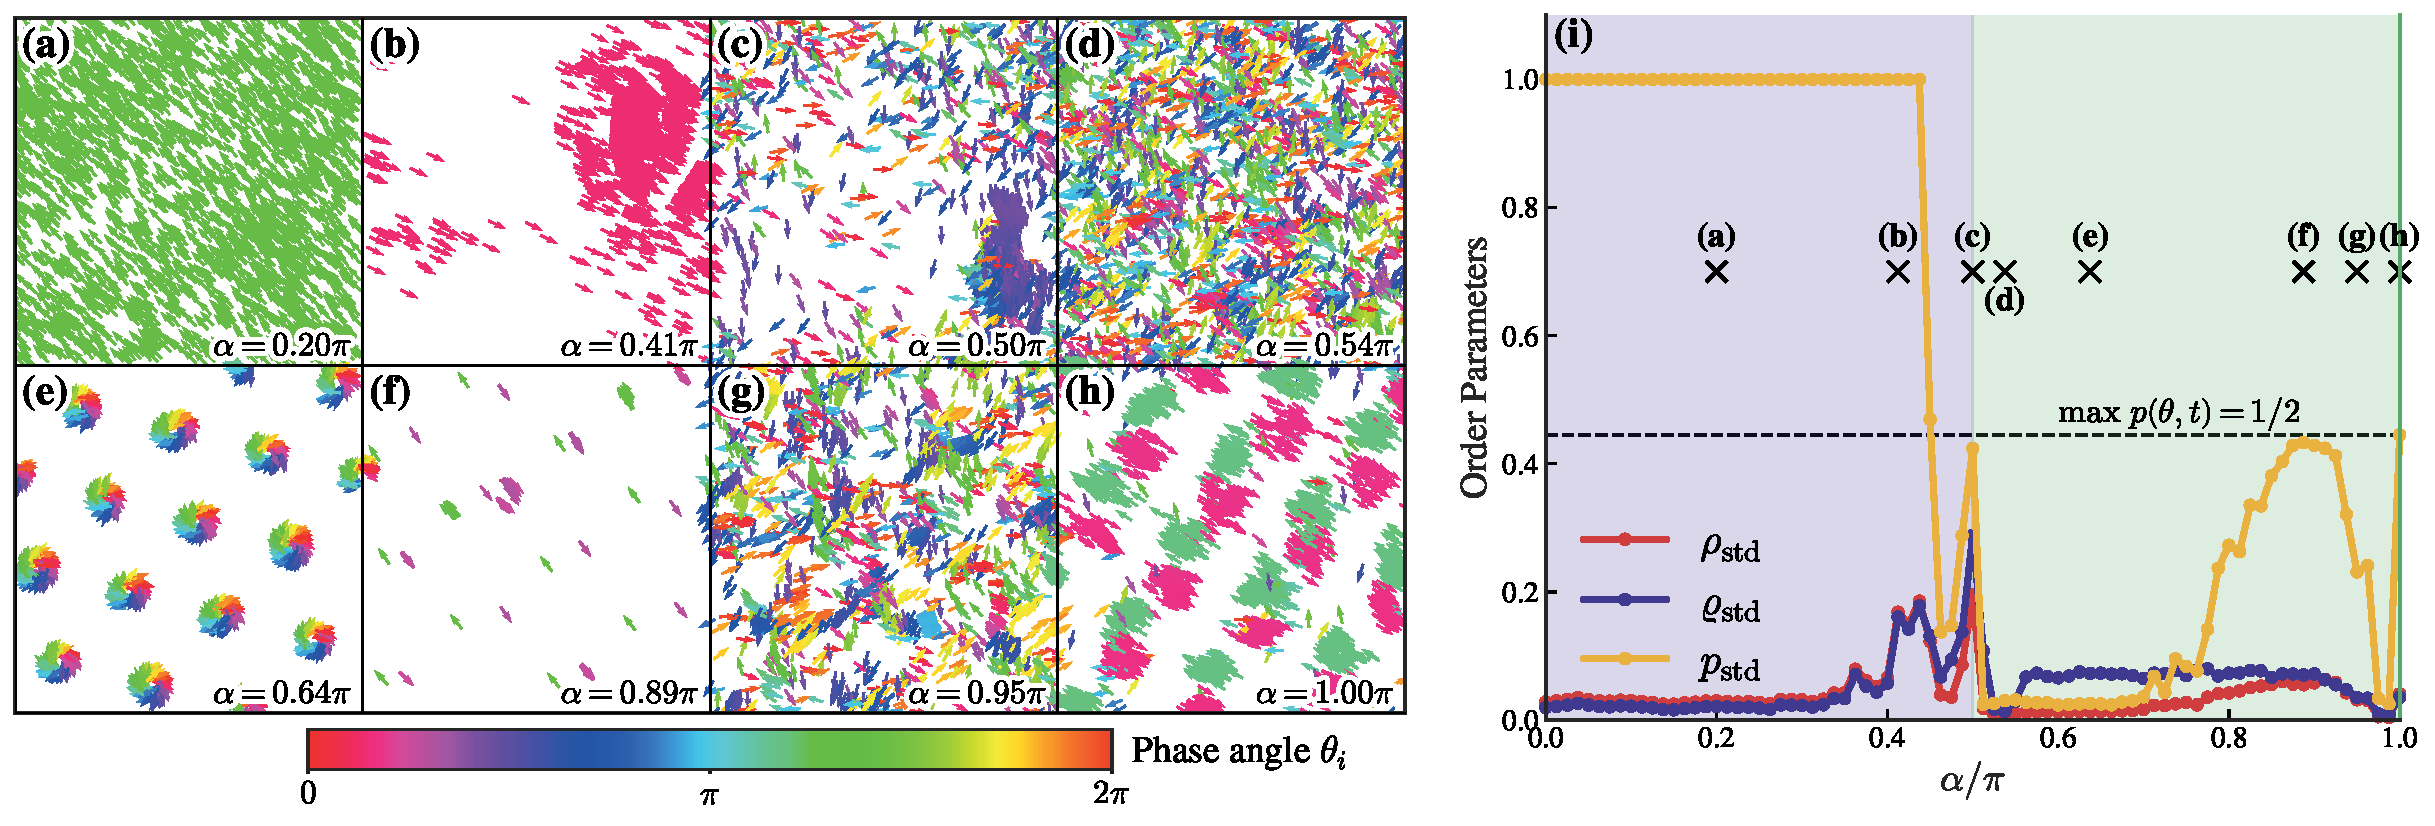
\includegraphics[width=\textwidth]{./figs/snapshotsAndPhaseDiagram.pdf}
    \caption{
        (a)-(h) Representative simulation snapshots for synchronization state [(a), (b)] and disordered state [(c), (d), (g)] and lattice state [(e), (f), (h)] at different phase frustration $\alpha$. The orientation and color of particles represent their instantaneous phase $\theta_i$.
        (i) Phase diagram and order parameters of the system with respect to the phase frustration $\alpha$. The crosses mark the snapshots in (a)-(h). Regions of blue, yellow and green (with single point $\alpha/\pi=1$) respectively represent the synchronized, nonuniform disordered, uniform disordered and lattice states.  
    }
\end{figure}

% \vspace{l}

% \begin{figure}[H]
%     \centering
%     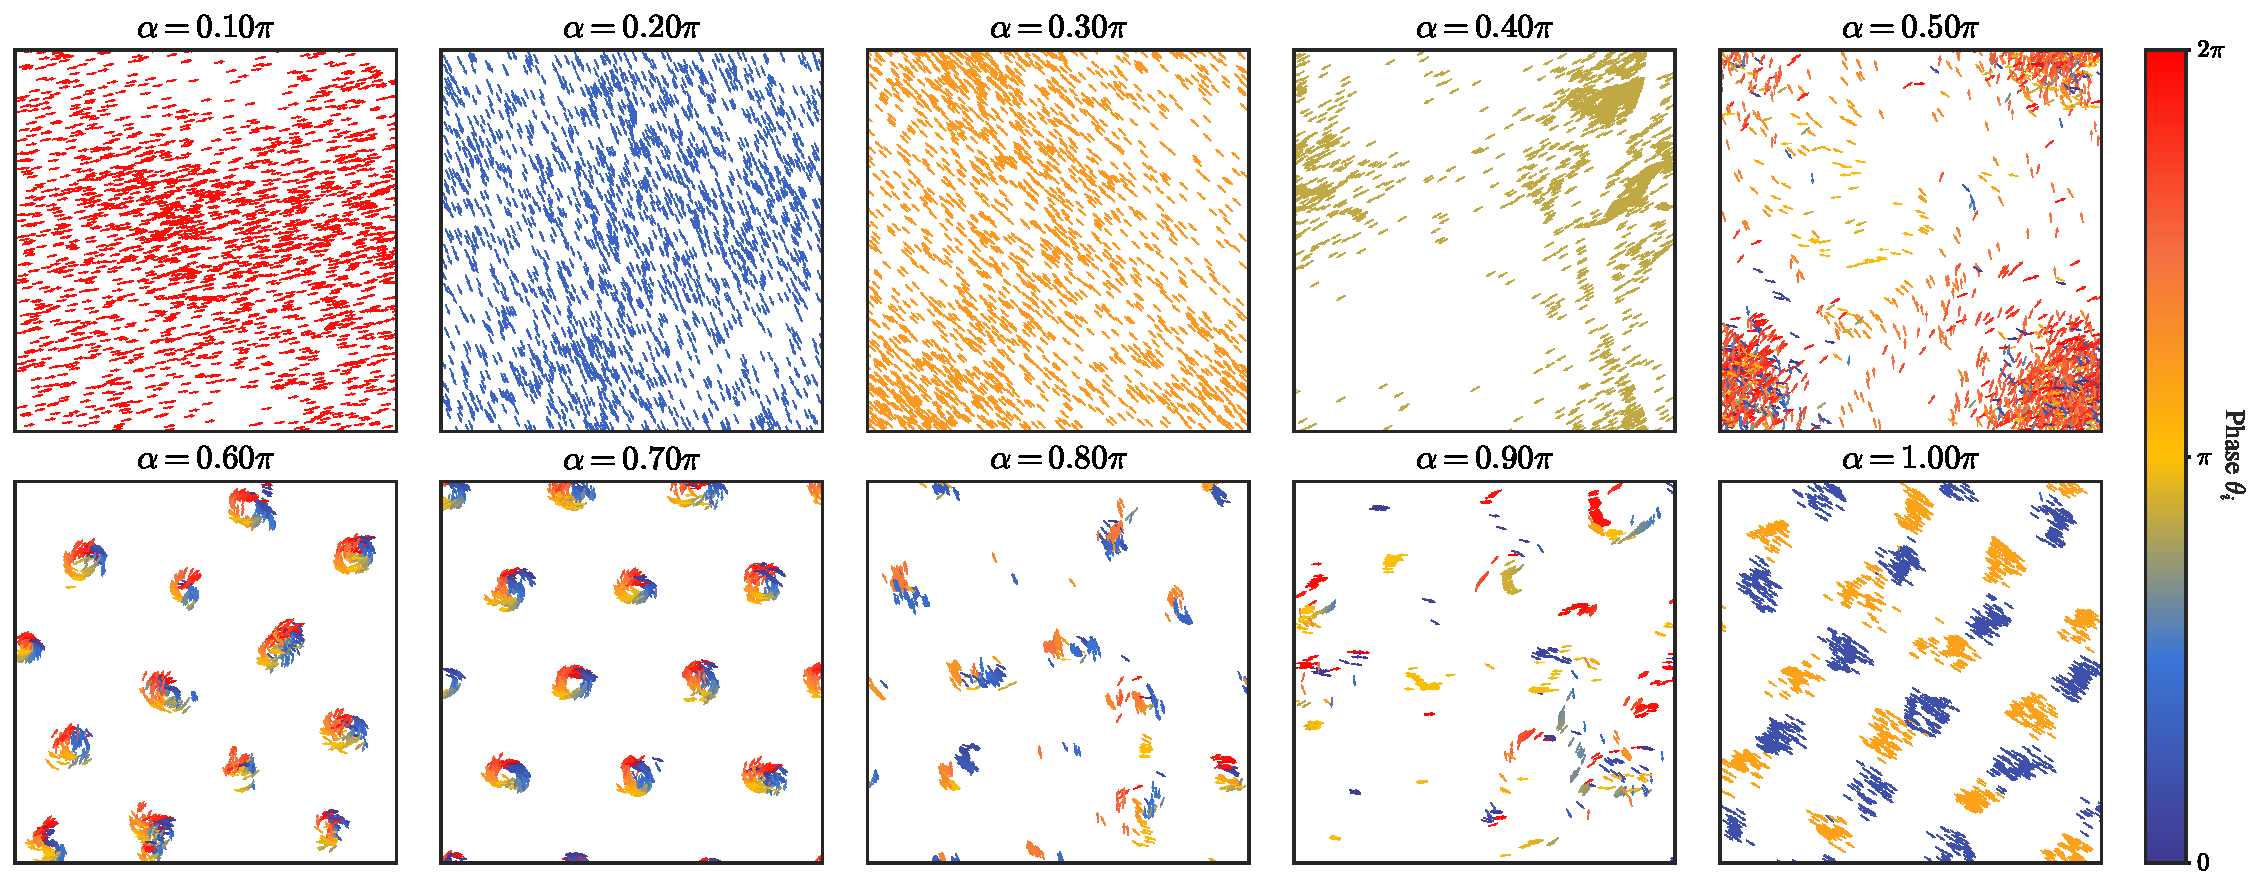
\includegraphics[width=\textwidth]{./figs/snapshot_v_alpha_K16.83_d01.55.pdf}
%     \caption{
%         Snapshot of the achiral system ($\omega _{\min}=0$, $\Delta \omega=0$) at $t=200$ with $N=2000$, $K=16.83$, and $d_0=1.55$.
%     }
% \end{figure}

\begin{figure}[H]
    \centering
    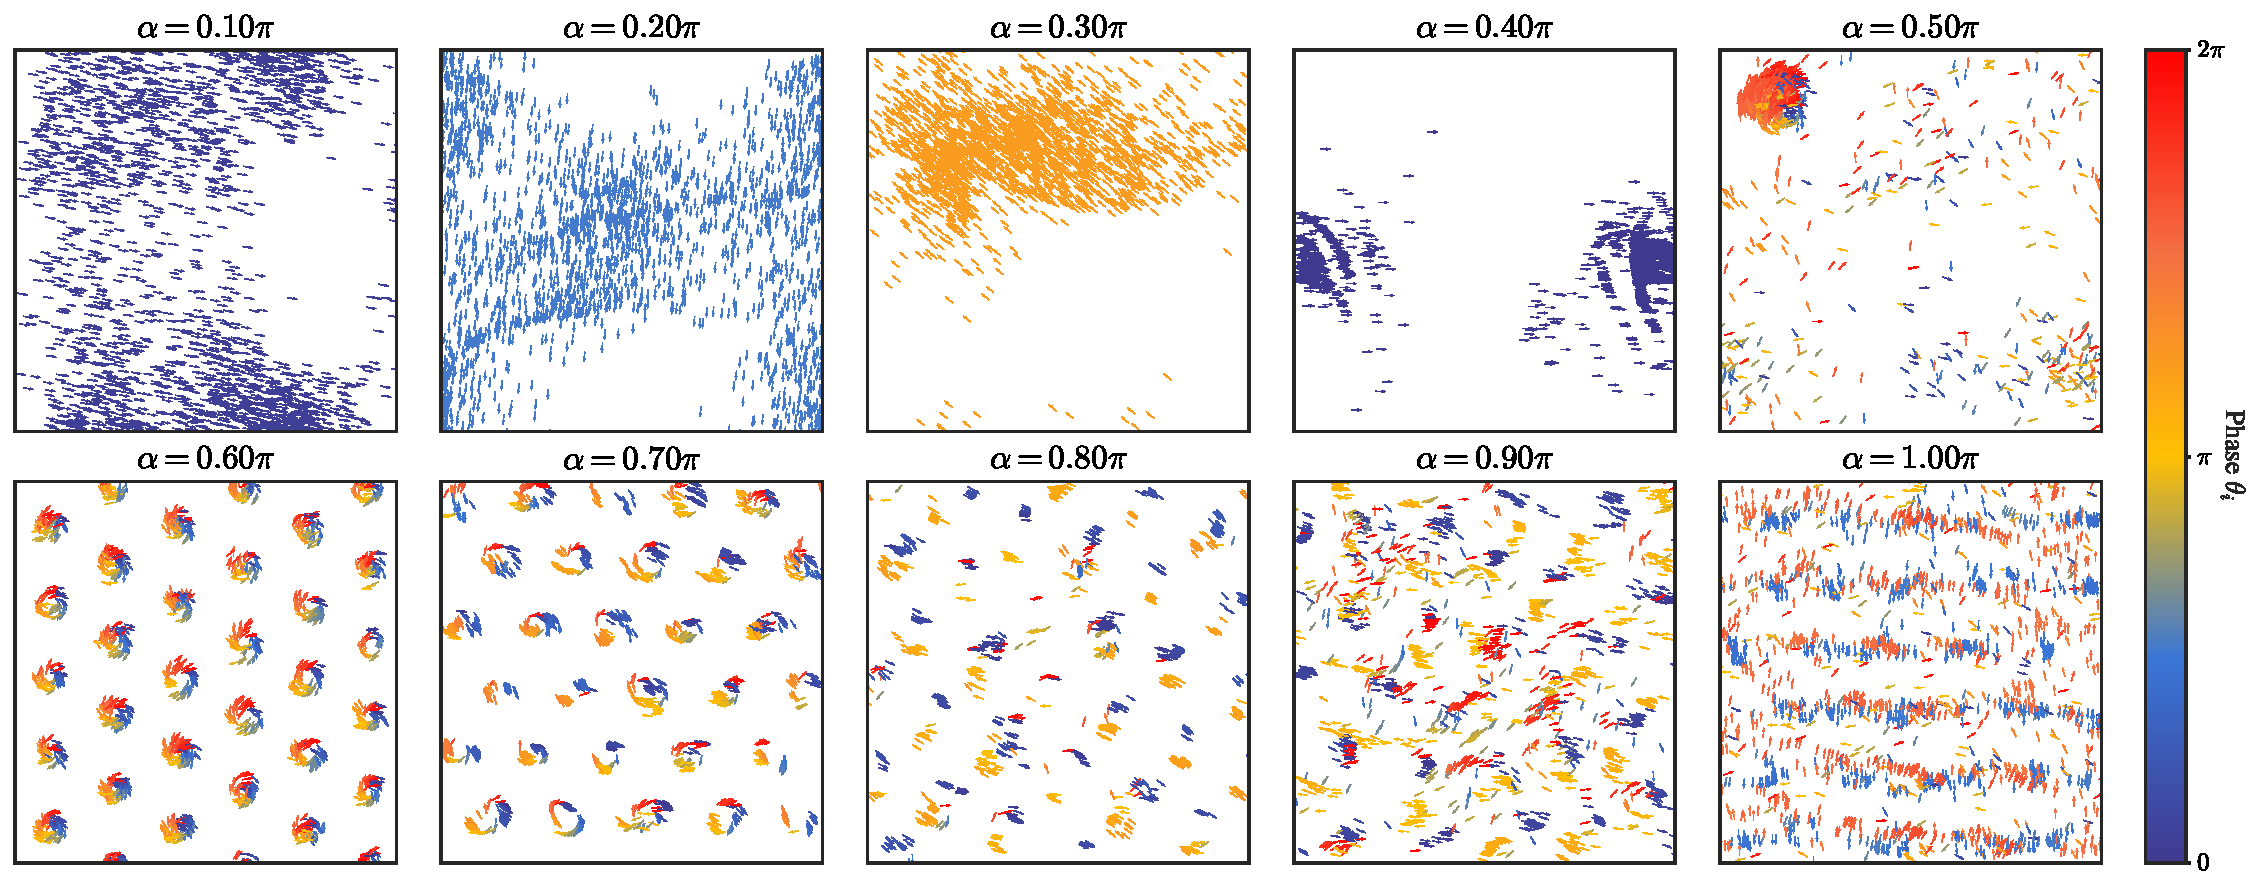
\includegraphics[width=\textwidth]{./figs/snapshot_v_alpha_K20.00_d01.00.pdf}
    \caption{
        Snapshot of the achiral system ($\omega _{\min}=0$, $\Delta \omega=0$) at $t=200$ with $N=2000$, $K=20$, and $d_0=1$.
    }
\end{figure}

\newpage
The phase diagram of the system is constructed by varying the key parameters, including the coupling strength $K$, the radius $d_0$. The resulting patterns are classified into ordered and lattice states. 

Single chirality particles can also form a triangular lattice structure:
\begin{figure}[H]
    \centering
    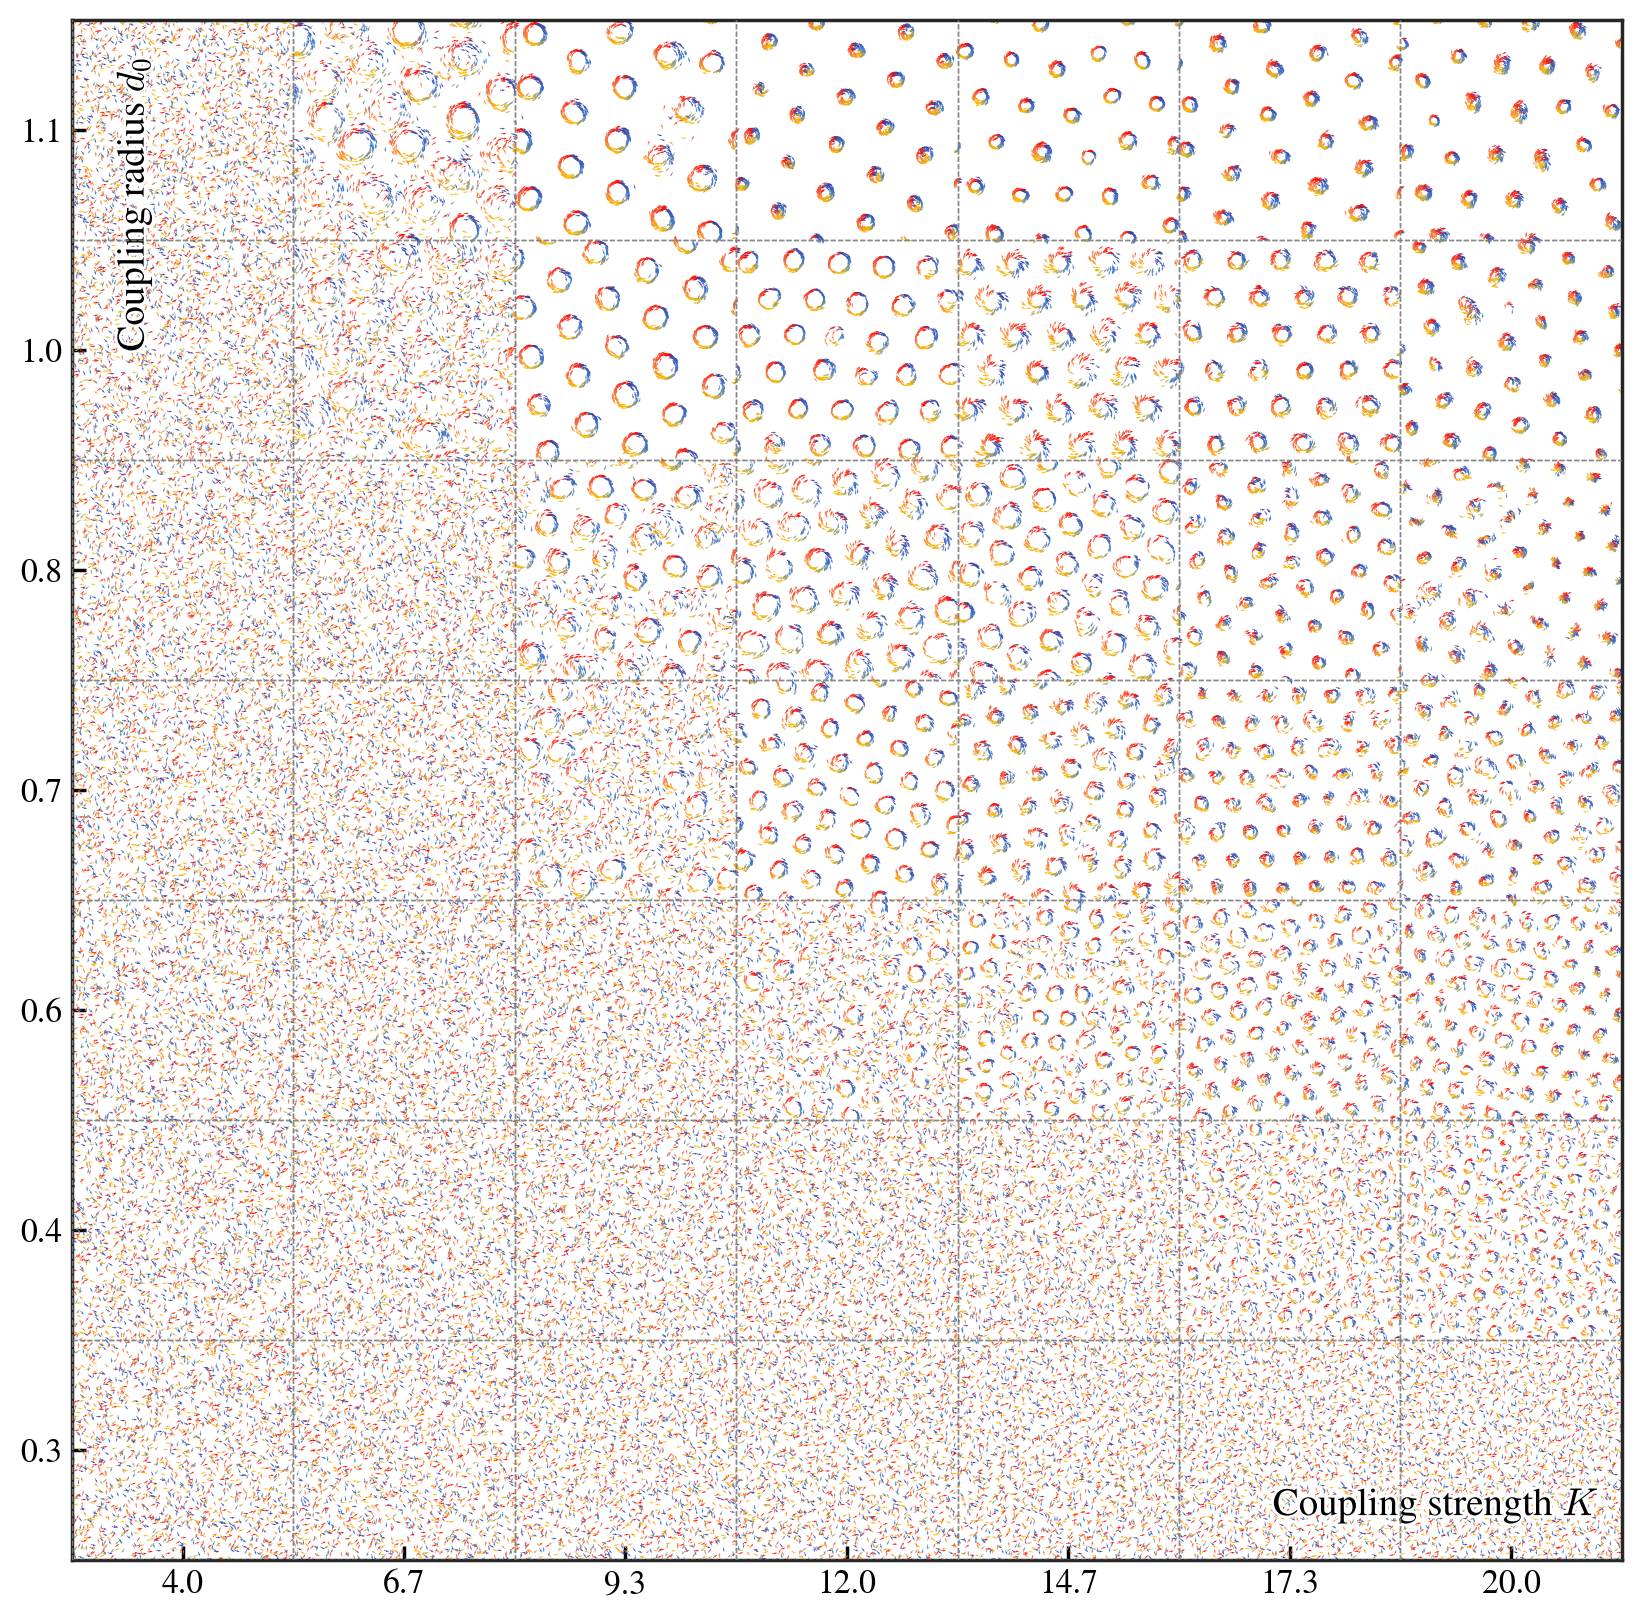
\includegraphics[width=0.9\textwidth]{./figs/asymmetric.png}
    \caption{
        Snapshots of asymmetric chiral system ($\omega _{i}\sim[0, 2]$) at different coupling strengths $K$ and radius $d_0$ for $\alpha = 0.6\pi$.
    }
\end{figure}
\vspace{-0.5cm}
\begin{figure}[H]
    \centering
    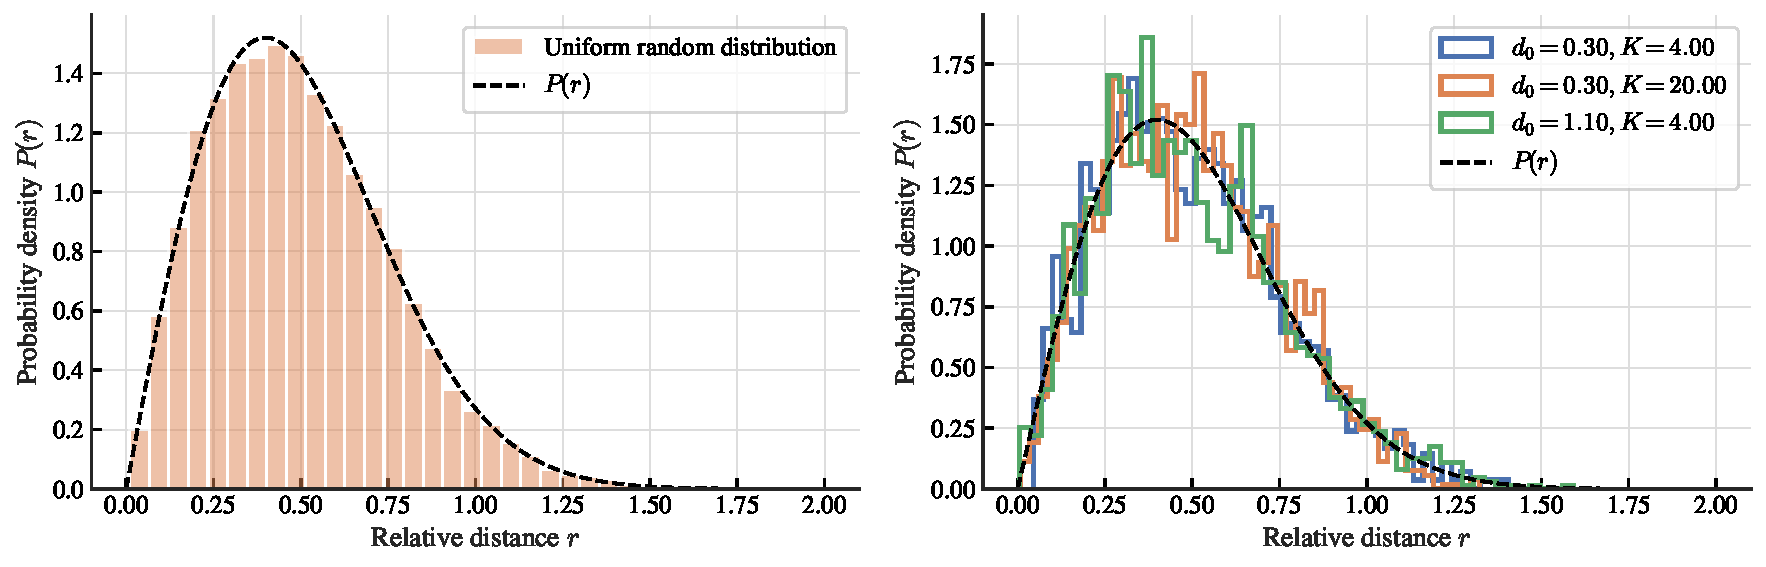
\includegraphics[width=0.9\textwidth]{./figs/uniform.pdf}
    \caption{
        The probability distribution functions (PDF) of distances, $r$, normalized with the mean particle spacing, $r_0$.
        The dash line is the PDF of Rayleigh Distribution $P(r)=2\pi r\exp\left[-\pi r^2\right]$.
    }
\end{figure}

\begin{figure}[H]
    \centering
    \includegraphics[width=\textwidth]{./figs/snapshot0.6pi.pdf}
    \caption{
        Snapshots of achiral system ($\omega _{\min}=0$ and $\Delta \omega=0$) at different coupling strengths $K$ and radius $d_0$ for $\alpha = 0.6\pi$. 
    }
\end{figure}

\begin{figure}[H]
    \centering
    \includegraphics[width=\textwidth]{./figs/PhaseLagPatternFormation_varying_strengthK_and_distanceD0_phase_a3.14_Do0_aN2000_distuniform.pdf}
    \caption{
        Snapshots of achiral system ($\omega _{\min}=0$ and $\Delta \omega=0$) at different coupling strengths $K$ and radius $d_0$ for $\alpha = \pi$. 
    }
\end{figure}

\begin{figure}[H]
    \centering
    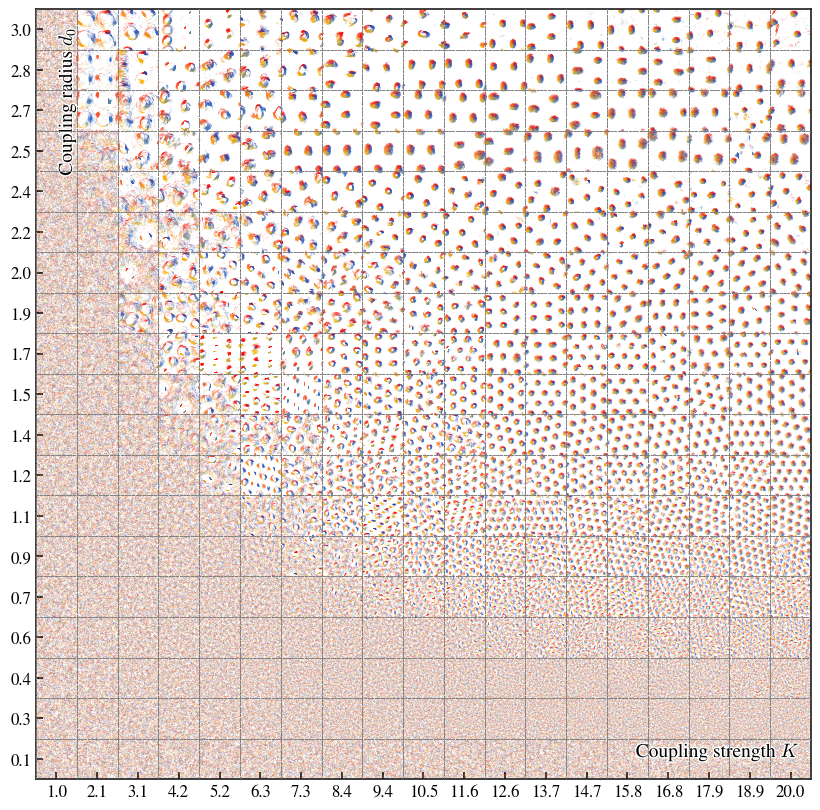
\includegraphics[width=\textwidth]{./figs/PhaseLagPatternFormation_varying_strengthK_and_distanceD0_phase_a1.88_Do0_aN2000_distuniform.png}
    \caption{
        \label{fig:snapshot0.6pi_chiral}
        Snapshots of achiral system ($\omega _{\min}=0$ and $\Delta \omega=0$) at different coupling strengths $K$ and radius $d_0$ for $\alpha = 0.6\pi$ with higher granularity. 
    }
\end{figure}

\begin{figure}[H]
    \centering
    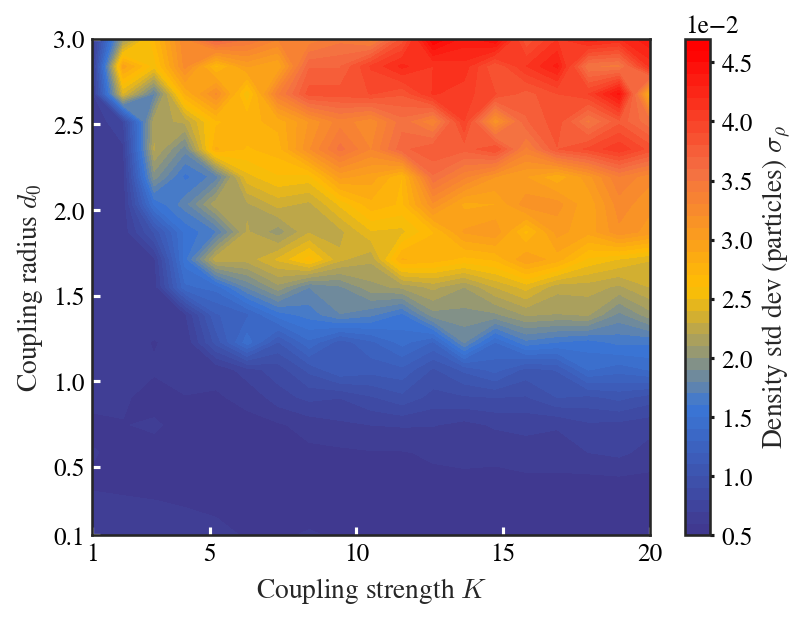
\includegraphics[width=0.7\textwidth]{./figs/orderParameter_varying_strengthK_and_distanceD0.png}
    \caption{
        \label{fig:orderParameter_varying_strengthK_and_distanceD0}
        The order parameter $\sigma _{\rho}\left( t \right)$ as a function of coupling strength $K$ and radius $d_0$(Corresponding to Fig.~\ref{fig:snapshot0.6pi_chiral}). The color indicates the value of the order parameter.
    }
\end{figure}

\newpage
\subsubsection{Respiration-like motion of unit cells}

For $\alpha=0.6\pi$, the system exhibits the respiration-like motion of the cells. Since the phases of particles in each cell are uniformly distributed in $[0, 2\pi]$ and the distance between cells is large enough to be considered decoupled, the effective frequency of each particle can be approximated by
\begin{equation}
    \dot{\theta}_i=-K\sin \alpha +\frac{K}{\left| A_i \right|}\int_0^{2\pi}{\mathrm{d}\theta ^{\prime}\sin \left( \theta ^{\prime}-\theta _i+\alpha \right)}=-K\sin \alpha\;,
\end{equation}
and the lattice constant $a$ can be approximated as 
\begin{equation}
    a=d_0+2\frac{v}{K\left| \sin \alpha \right|}\;.
    \label{eq:latticeConstant}
\end{equation}
\begin{figure}[H]
    \centering
    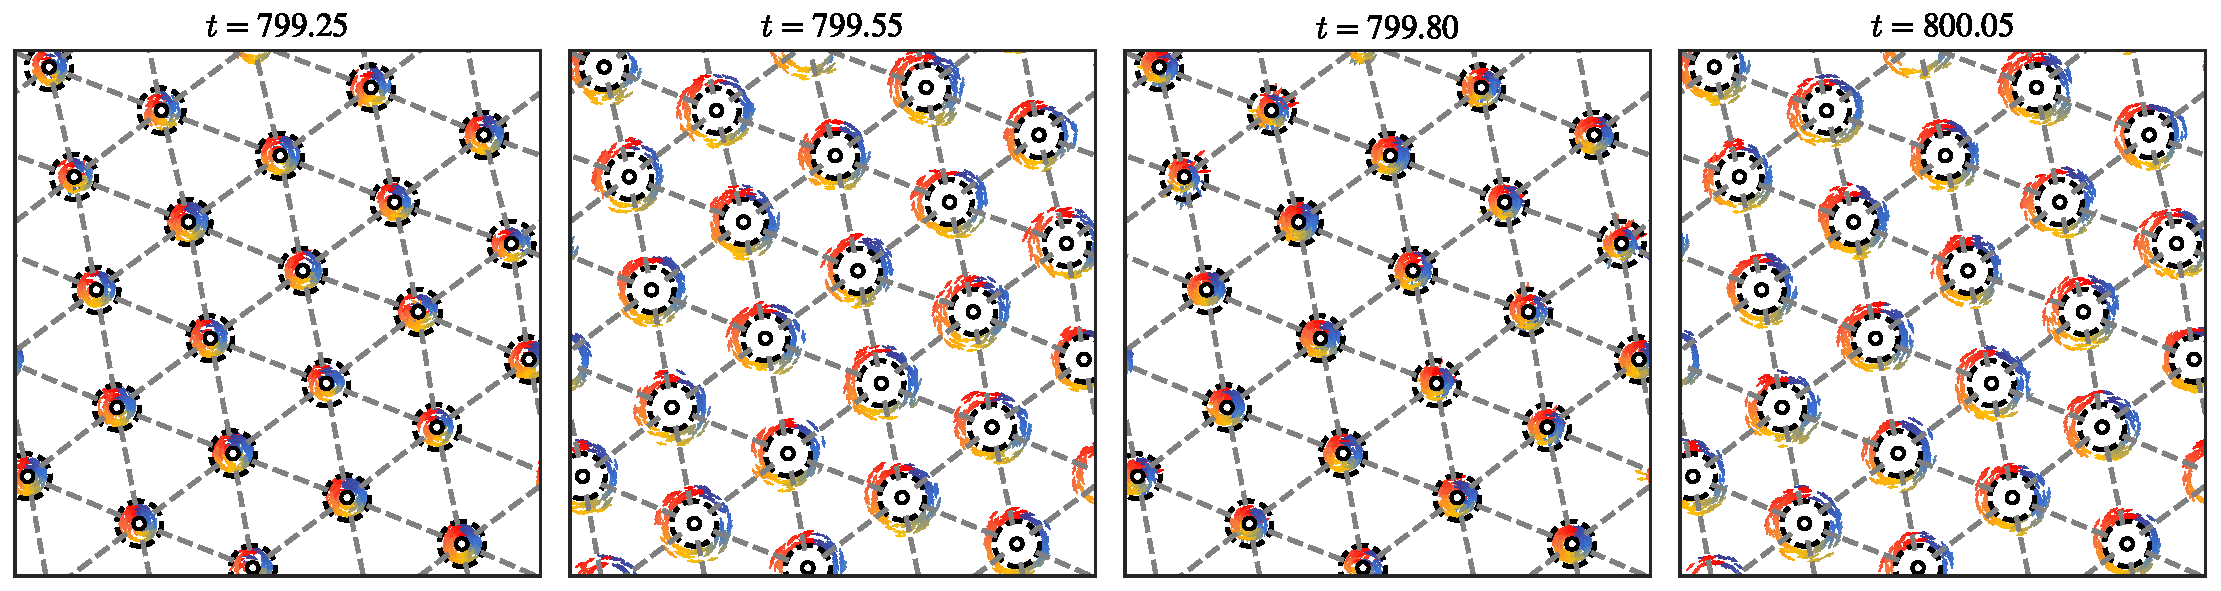
\includegraphics[width=\textwidth]{./figs/respiration_snapshot.pdf}
    \caption{
        \label{fig:respiration_snapshot}
        respiration-like motion of the cells with $\omega _{\min}=0$, $\Delta \omega=0$, $N=3000$, $K=10.5$, $d_0=1.07$, and $\alpha=0.6\pi$. Black hollow dots represent the center of mass of each cell, black dash circles represent the theoretical unit cell radius $v/\dot{\theta}_i$, and the gray dash lines represent the theoretical distance between unit cells $d_0$.
    }
\end{figure}
\begin{figure}[H]
    \centering
    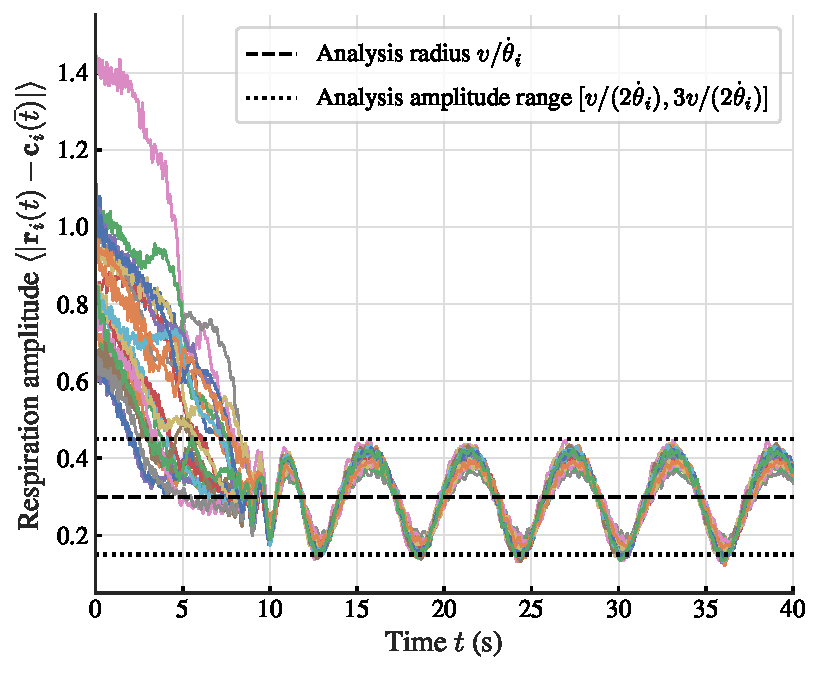
\includegraphics[width=0.5\textwidth]{./figs/respiration_amplitude.pdf}
    \caption{
        \label{fig:respiration_amplitude}
        respiration amplitude of the system. 
        The parameters are the same as in Fig.~\ref{fig:respiration_snapshot}.
        Different colors represent different cells, and the amplitude is defined as the distance between particles and the center of mass of the cell at final state ($\bar{t}=40$).
    }
\end{figure}
As shown in Fig.~\ref{fig:respiration_snapshot} and Fig.~\ref{fig:respiration_amplitude}, the respiration amplitude of the cells is defined as $\left< \left| \mathbf{r}_i\left( t \right) -\mathbf{c}_i\left( \bar{t} \right) \right| \right> $, where $\mathbf{c}_i(\bar{t})$ is the center of mass of the cell of $i$-th particle at final state ($\bar{t}=40$), and $\left< \cdot \right>$ denotes the average over all particles in the cell. It is worth noting that the amplitude is fluctuating around the theoretical cell radius $v/\dot{\theta}_i$ and the
respiration frequency of the cells exhibit synchronization.

\begin{figure}[H]
    \centering
    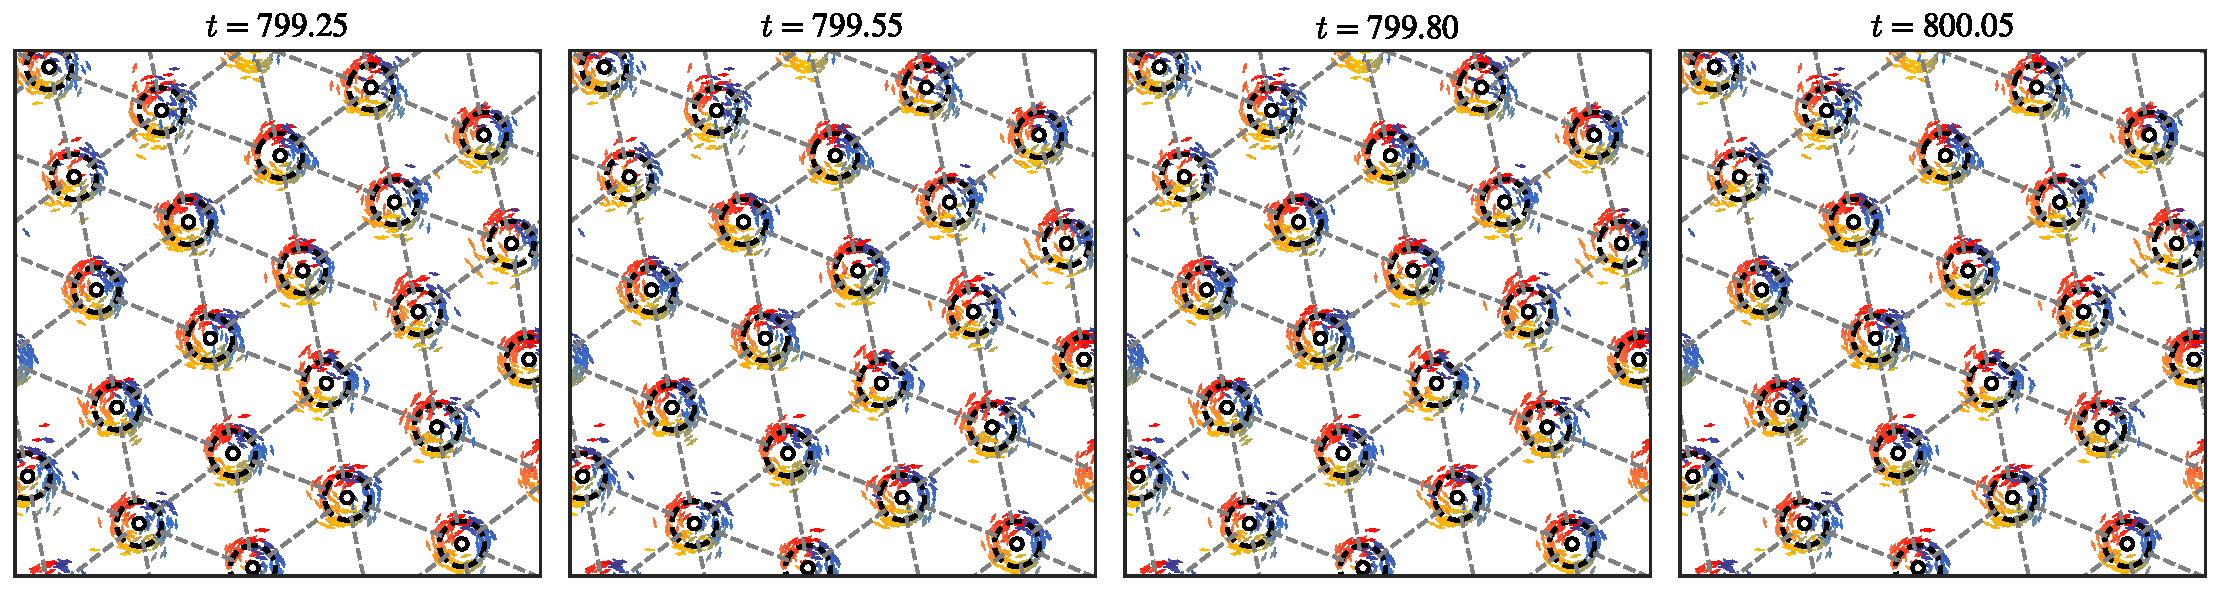
\includegraphics[width=\textwidth]{./figs/respiration_snapshot_decoupled.pdf}
    \caption{
        respiration-like motion of the decoupled cells. The parameters are the same as in Fig.~\ref{fig:respiration_snapshot}.
    }
\end{figure}

\begin{figure}[H]
    \centering
    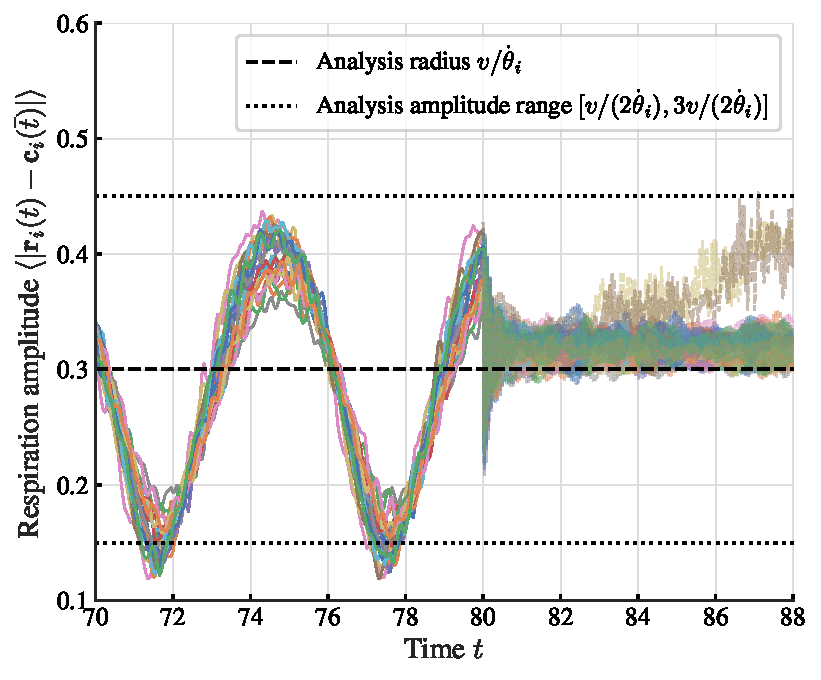
\includegraphics[width=0.5\textwidth]{./figs/respiration_amplitude_cells_decouled.pdf}
    \caption{
        Respiration amplitude of the decoupled cells ($t > 80$). The parameters are the same as in Fig.~\ref{fig:respiration_snapshot}.
    }
\end{figure}

\newpage
\subsubsection{Lattice constant}

\begin{figure}[H]
    \centering
    \subcaptionbox{
        Continuous spectrum $\mathrm{Re}[ \lambda _{m}^{\left[ 0 \right]}\left( k \right) ]$ as a function of wave number $k$ for $K=20, d_0=1$.
    }[0.49\linewidth]{
        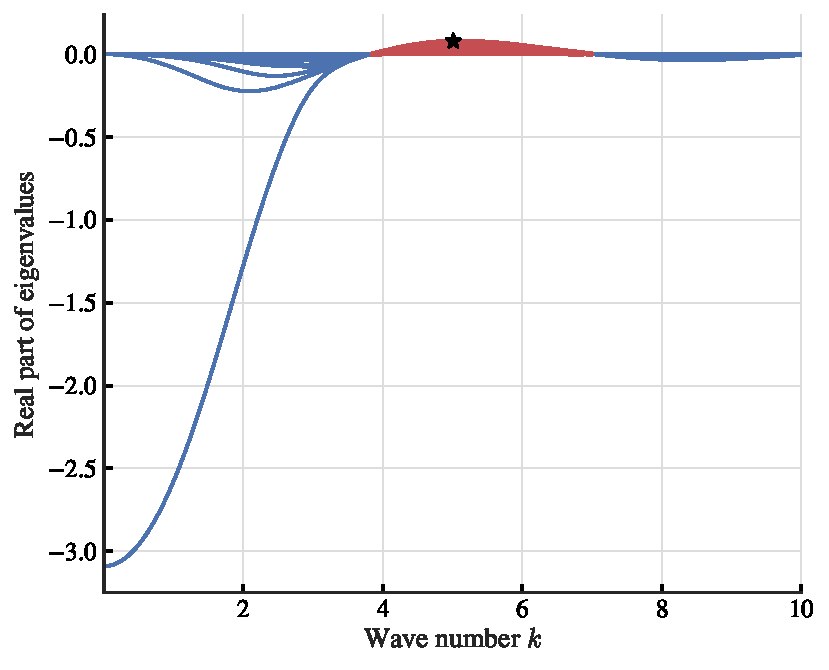
\includegraphics[width=\linewidth]{./figs/continuous_spectrum.pdf}
    }
    \hfill
    \subcaptionbox{
        Mean lattice constant $a$ versus the most unstable wave number $k^*$ (defined as the maximum point of $\mathrm{Re}[ \lambda _{m}^{\left[ 0 \right]}\left( k \right) ]$).
    }[0.49\linewidth]{
        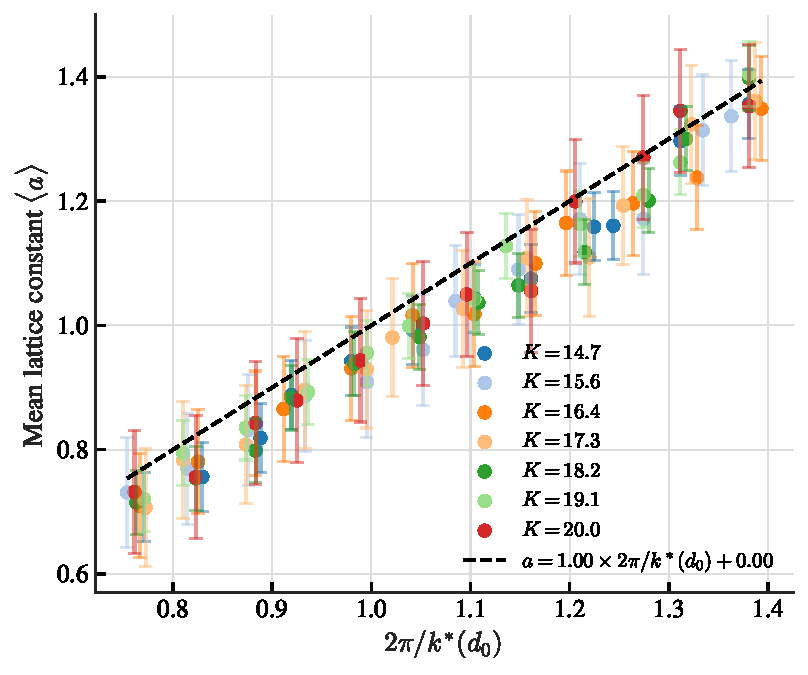
\includegraphics[width=\linewidth]{./figs/lattice_constant_vs_kstar.pdf}
    }
    \caption{
        Lattice constant $a$ as a function of coupling strength $K$ and radius $d_0$ for $\alpha=0.6\pi$.
    }
\end{figure}

\newpage
\subsubsection{Initial conditions determined cells composition \label{sec:cellComposition}}

\begin{figure}[H]
    \centering
    \subcaptionbox{Initial conditions of half on each side.}[0.49\linewidth]{
      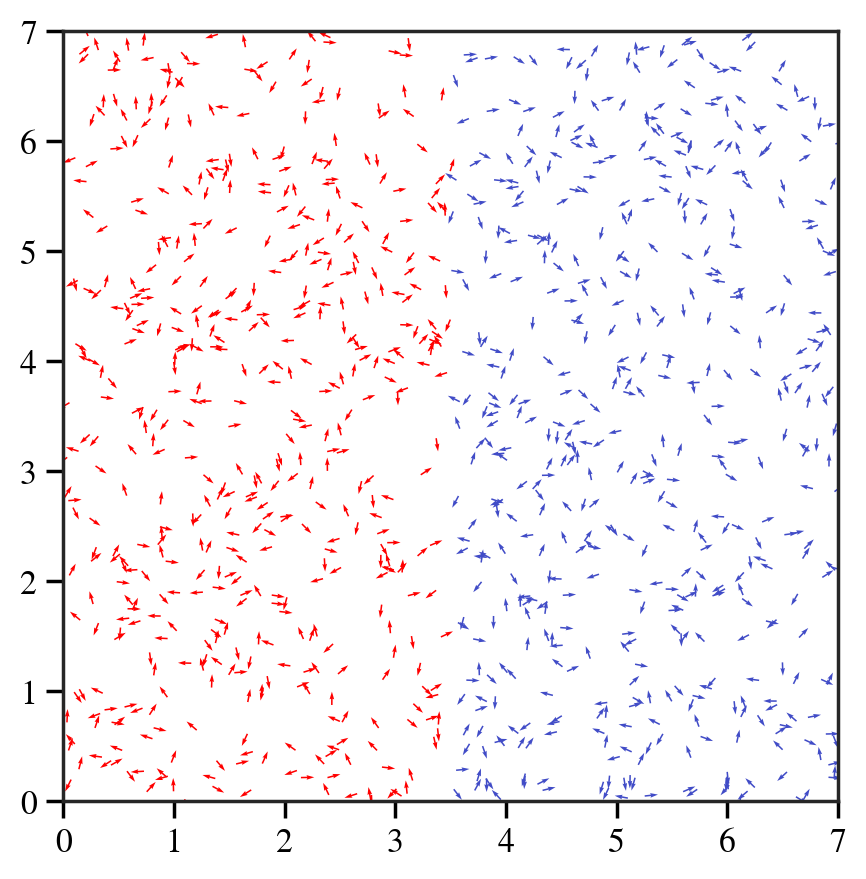
\includegraphics[width=\linewidth]{figs/halfSide.png}
    }
    \hfill
    \subcaptionbox{
        Initial conditions of chessboard pattern.
    }[0.49\linewidth]{
      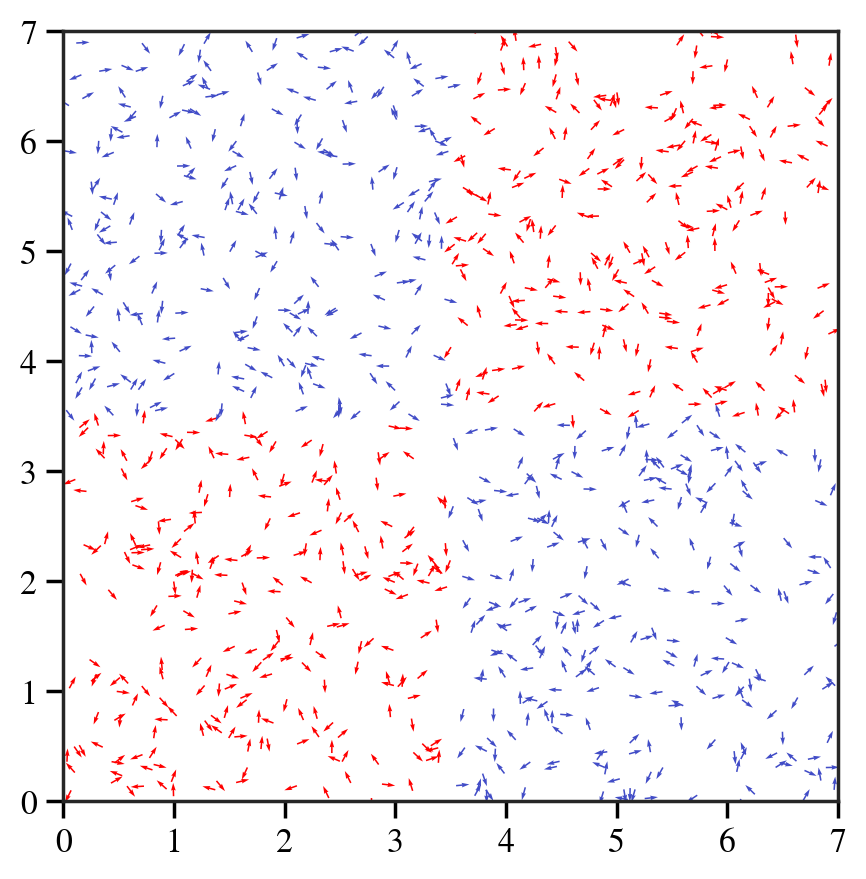
\includegraphics[width=\linewidth]{figs/chess.png}
    }
    \caption{
        Two artificial non-uniform initial conditions in space. Red and blue particles represent particles with positive and negative chirality, respectively. 
    }
\end{figure}

\begin{figure}[H]
    \centering
    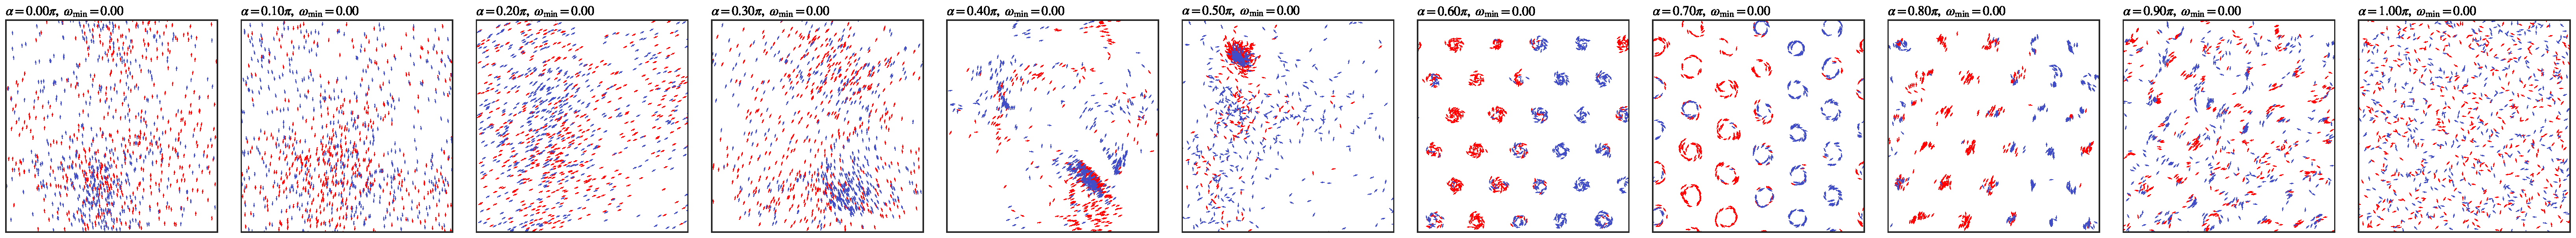
\includegraphics[width=\textwidth]{./figs/HalfInitPhaseLagPatternFormation_a0.00_Do1_aN1000_distuniform.pdf}
    \caption{
        \label{fig:half}
        Snapshot of the system at $t=80$ with $N=1000$, $K=20$, $\omega _{\min}=0$, $\Delta \omega=1$ and initial conditions of half on each side.
    }
\end{figure}

\begin{figure}[H]
    \centering
    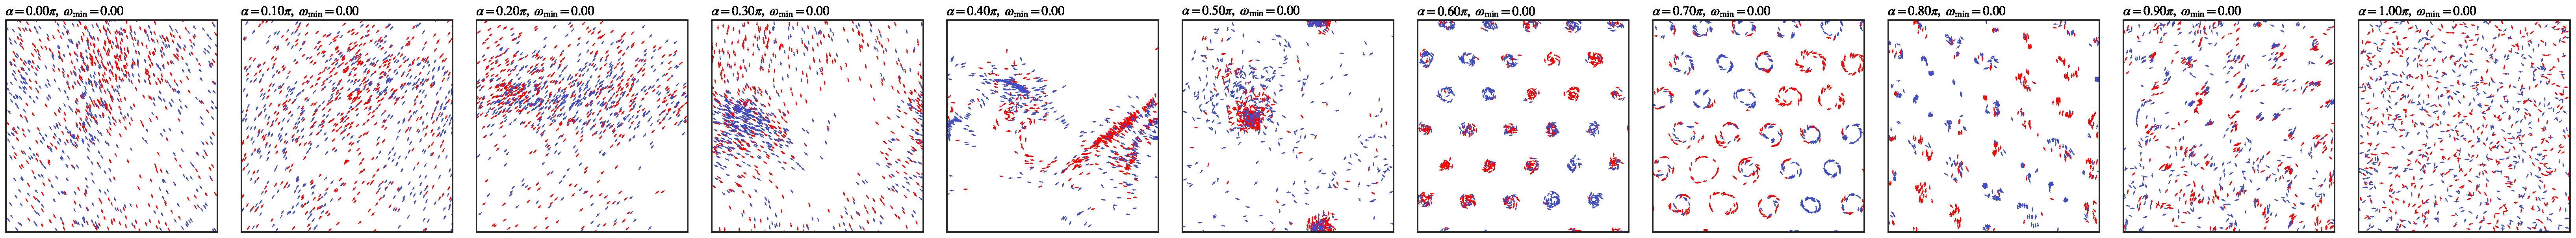
\includegraphics[width=\textwidth]{./figs/ChessboardPhaseLagPatternFormation_a0.00_Do1_aN1000_distuniform.pdf}
    \caption{
        \label{fig:chess}
        Snapshot of the system at $t=80$ with $N=1000$, $K=20$, $\omega _{\min}=0$, $\Delta \omega=1$ and initial conditions of chessboard pattern.
    }
\end{figure}

\newpage

% \begin{figure}[H]
%     \centering
%     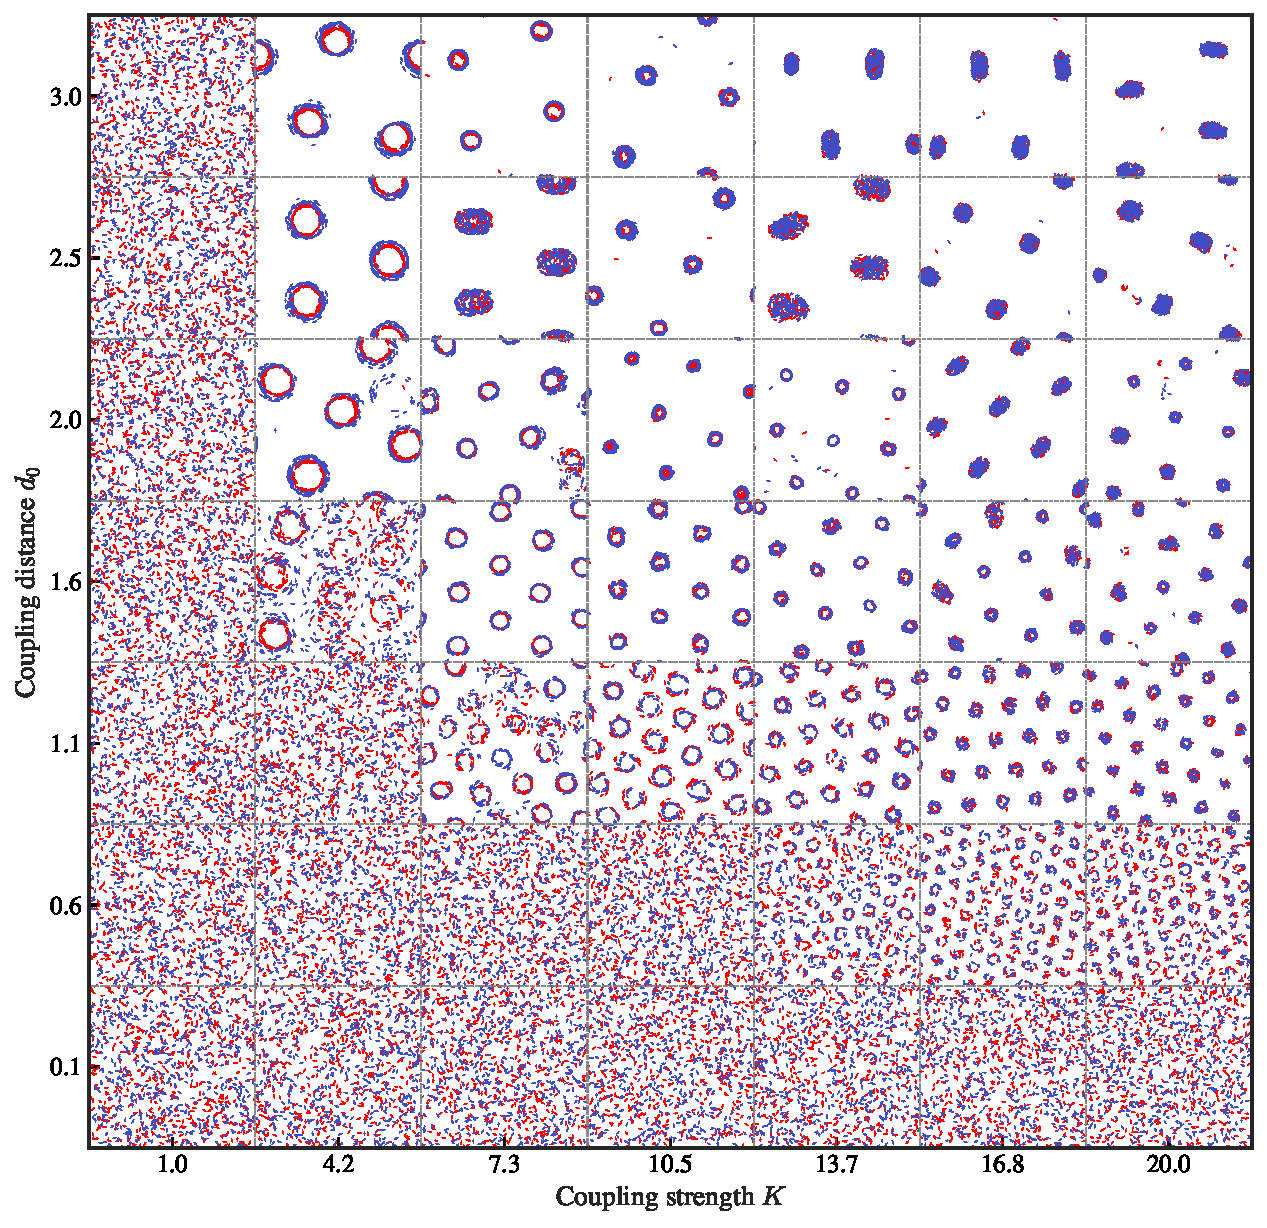
\includegraphics[width=0.75\textwidth]{./figs/PhaseLagPatternFormation_varying_strengthK_and_distanceD0_freq_a1.88_Do1_aN1000.pdf}
%     \caption{
%         \label{fig:snapshot0.6pi_chiral}
%         Snapshots of system at different coupling strengths $K$ and radius $d_0$ with $N=1000$, $K=20$, $\alpha =0.6\pi$, $\omega _{\min}=0$, and $\Delta \omega =1$. 固定阻锉为$0.6\pi$,不同的耦合强度$K$和半径$d_0$下的手性粒子系统快照。粒子颜色根据其瞬时相位$\theta_i$着色。随着两个耦合参数的增加,粒子在空间中逐渐形成三角晶格结构且尺寸和彼此距离不断增加。
%     }
% \end{figure}

% \begin{figure}[H]
%     \centering
%     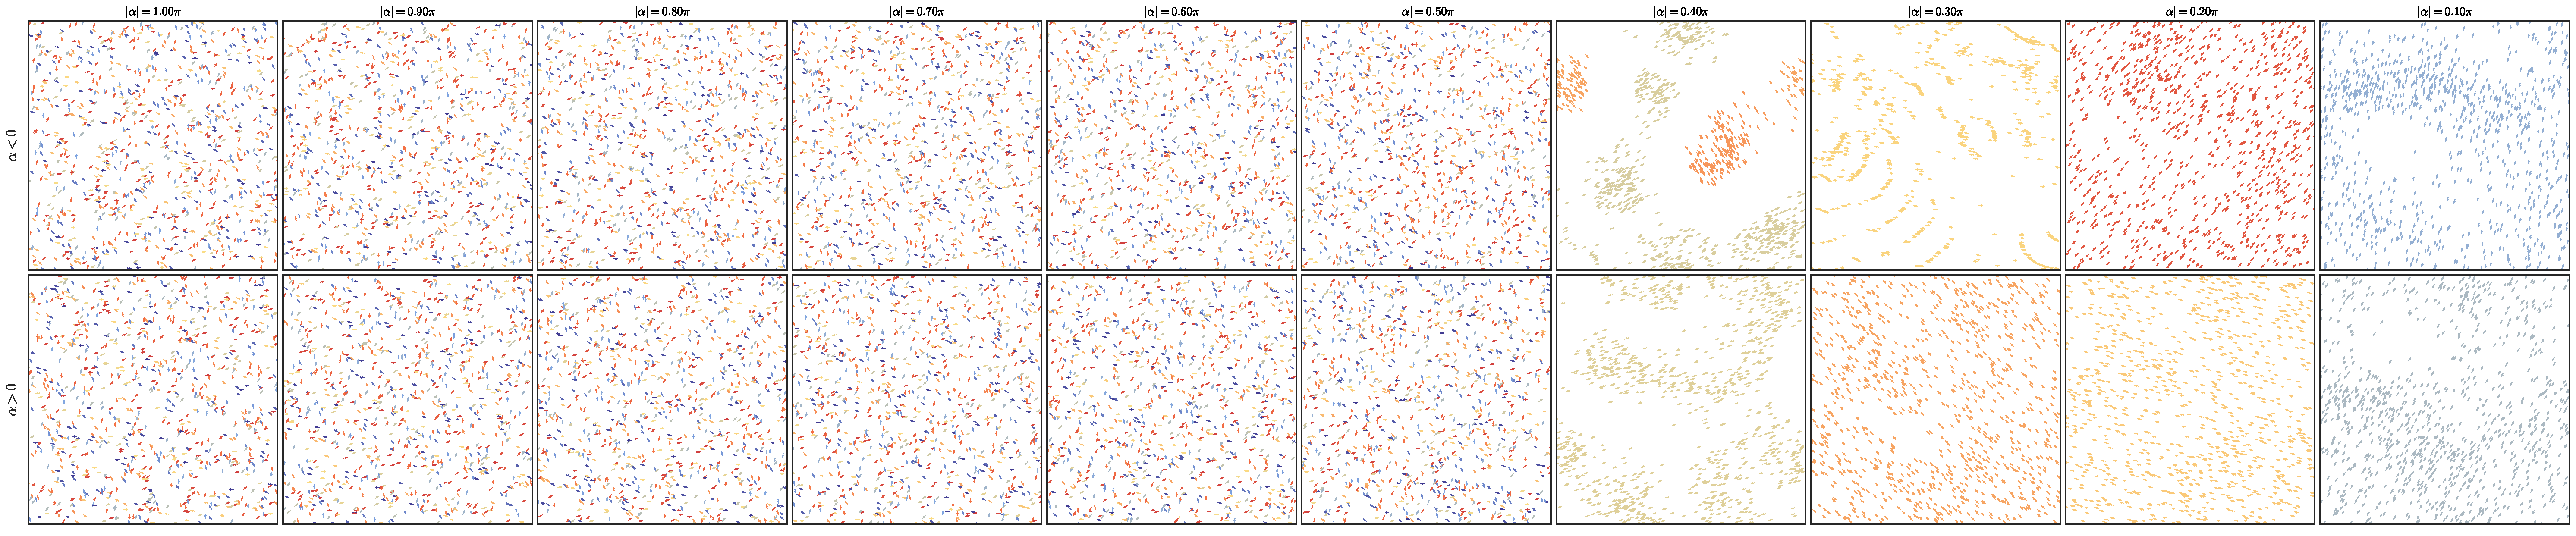
\includegraphics[width=\textwidth]{./figs/noncounter_snapshot.pdf}
%     \caption{
%         Snapshot of the system without counter term $-\sin\alpha$ at $t=80$ with $N=1000$, $K=20$, $\omega _{\min}=0.1$ and $\Delta \omega=1$. The particles are colored according to their instantaneous phase $\theta_i$. There is no triangular lattice structure, and the particles are randomly distributed in space.
%         系统终态的快照,粒子颜色根据其瞬时相位$\theta_i$着色。空间排列没有三角晶格结构,粒子在空间中随机分布。
%     }
%     \label{fig:noncounter_shotsnaps}
% \end{figure}

% \begin{figure}[H]  % 如果希望把图片放在当前段落中,可以使用[H]选项
%     \centering
%     \subcaptionbox{Snapshot}[0.49\linewidth]{
%       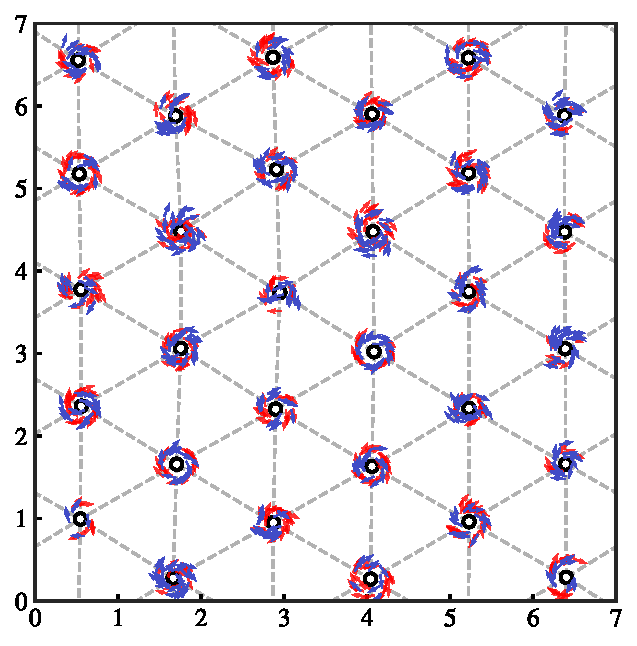
\includegraphics[width=\linewidth]{figs/snapshot.pdf}
%     }
%     \hfill
%     \subcaptionbox{
%         Statistics of cells
%     }[0.49\linewidth]{
%       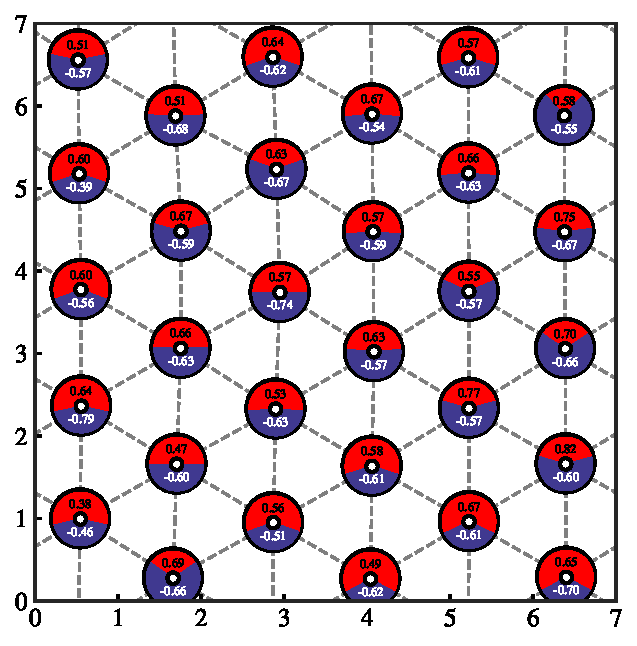
\includegraphics[width=\linewidth]{figs/statistics.pdf}
%     }
%     \caption{
%         Snapshot and statistics of cells of system at $t=80$ with $N=1000$, $K=20$, $\alpha =0.6\pi$, $\omega _{\min}=0.1$, and $\Delta \omega =1$. In \textbf{(b)}, the pie chart shows the proportion of two chiralities in the cell, and the black, white text indicates the mean natural frequency of positive, negative chiral particles in the cell, respectively.
%         系统终态的快照和晶格统计。快照中,粒子晶格呈现三角形晶格结构。饼图显示了正负两种粒子在晶格中的比例,黑色和白色文本分别表示正负粒子的平均自然频率。
%     }
% \end{figure}

% 陆羿辰:从统计结果中看不出临近晶格之间的规律,似乎和粒子数目以及粒子的自然频率无关。

% \begin{figure}[H]  % 如果希望把图片放在当前段落中,可以使用[H]选项
%     \centering
%     \subcaptionbox{
%         Colors represent the mean natural frequency
%     }[0.49\linewidth]{
%       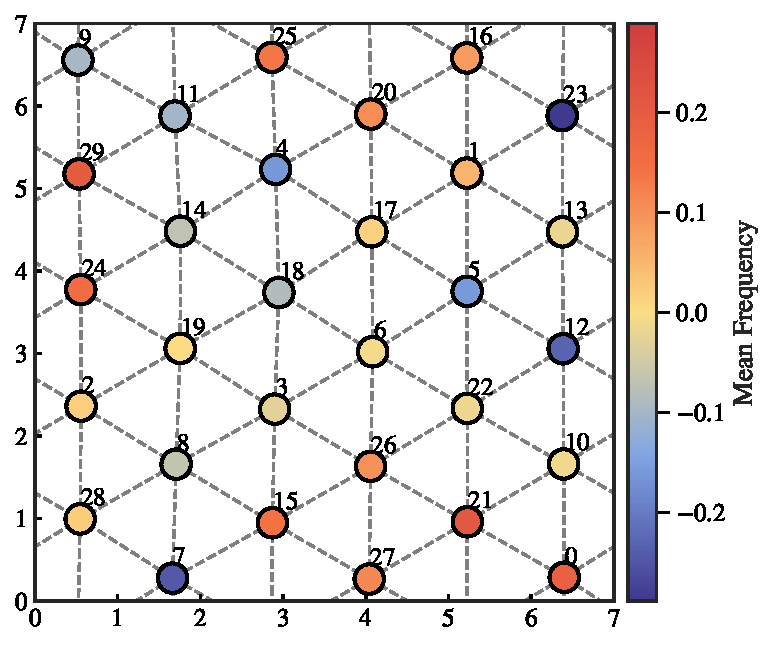
\includegraphics[width=\linewidth]{figs/mean_freq.pdf}
%     }
%     \hfill
%     \subcaptionbox{
%         Colors represent the mean effective frequency
%     }[0.49\linewidth]{
%       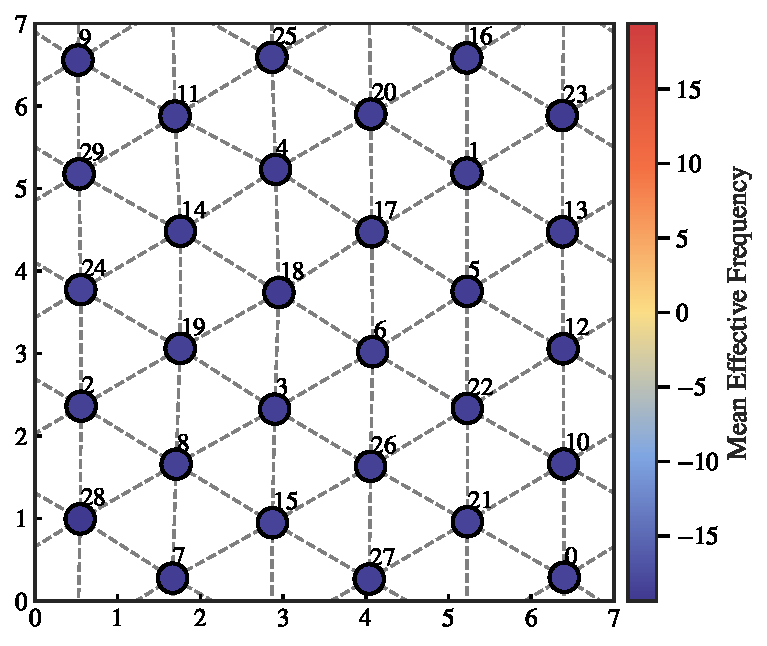
\includegraphics[width=\linewidth]{figs/mean_eff_freq.pdf}
%     }
%     \caption{
%         \label{fig:mean_freq}
%         The mean natural frequency and effective frequency of particles in each cell. The effective frequency is defined as the average instantaneous phase velocity of particles in the cell.
%         \textbf{(a)} shows the mean natural frequency of particles in each cell, while \textbf{(b)} shows the mean effective frequency of particles in each cell.
%         每个晶格中粒子的平均自然频率和有效频率。有效频率定义为晶格中粒子终态瞬时相速度的平均值。\textbf{(a)}显示了每个晶格中粒子的平均自然频率,而\textbf{(b)}显示了每个晶格中粒子的平均有效频率。
%     }
% \end{figure}

% \begin{figure}[H]
%     \centering
%     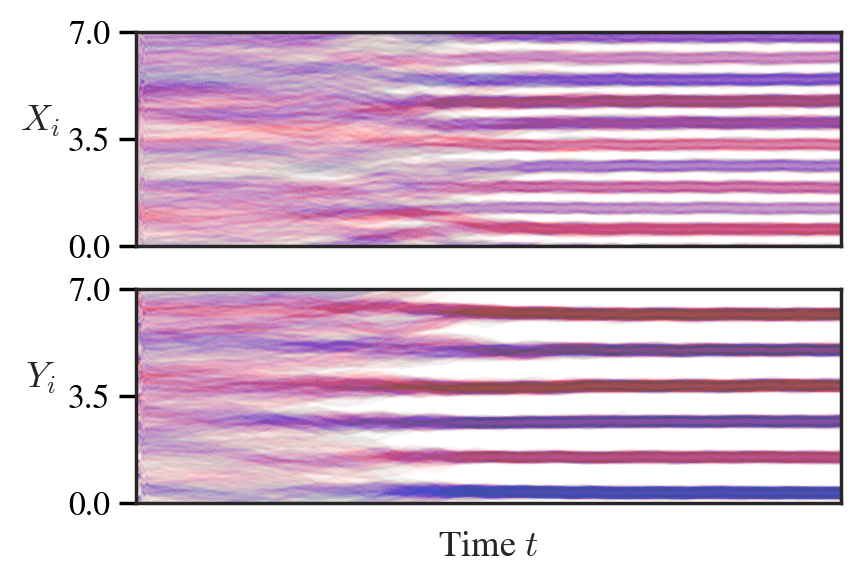
\includegraphics[width=0.6\textwidth]{./figs/Center Scatter.png}
%     \caption{
%        \label{fig:Center Scatter}
%        瞬时旋转中心随时间变化的散点图。其中$N=1000$, $K=20$, $\alpha =0.6\pi$,  $\omega _{\min}=0.1$。随时间演化,粒子晶格大体呈现红蓝交错分布的趋势。
%     }
% \end{figure}

\newpage
\section{Critical condition for phase transition and mechanism}

\subsection{Linear stability analysis with amplitude ansatz}

In the thermodynamic limit $N\to \infty$, the state of the system in Eq.~\eqref{eq:totalDynamicsMeanField} can be characterized by the single-oscillator distribution $\rho \left( \mathbf{r},\theta ,t \right) $, which satisfies the continuity equation
\begin{equation}
    \frac{\partial \rho}{\partial t}=-v\mathbf{p}\left( \theta \right) \cdot \nabla \rho -\frac{\partial}{\partial \theta}\left\{ \mathcal{T} \left[ \rho \right] \rho \right\} \;,
    \label{eq:globalContinuityEquation}
\end{equation}
where $\mathcal{T}$ is the linear operator that has the form
\begin{equation}
    \begin{aligned}
        \mathcal{T} \left[ \rho \right] =&\frac{K}{A}\int_{L\times L}{\mathrm{d}^2\mathbf{r}^{\prime}\int_0^{2\pi}{\mathrm{d}\theta ^{\prime}\rho \left( \mathbf{r}^{\prime},\theta ^{\prime},t \right)}}\\
        &\times \Theta \left( d_0 - \left| \mathbf{r}^{\prime}-\mathbf{r} \right| \right) \left[ \sin \left( \theta ^{\prime}-\theta +\alpha \right) -\sin \alpha \right]\;,
    \end{aligned}
\end{equation}
where $\Theta(r) $ is Heaviside step function and  
\begin{equation}
    A=\int_{L\times L}{\mathrm{d}^2\mathbf{r}^{\prime}\int_0^{2\pi}{\mathrm{d}\theta ^{\prime}\rho \left( \mathbf{r}^{\prime},\theta ^{\prime},t \right) \Theta \left( d_0 - \left| \mathbf{r}^{\prime}-\mathbf{r} \right|\right)}}\;.
\end{equation}

One obvious solution of Eq.~\eqref{eq:globalContinuityEquation} is $\rho=(2\pi L^2)^{-1}$ representing a uniform disordered state. The stability of such a solution can be investigated by considering a small perturbation,
\begin{eqnarray}
    \rho \left( \mathbf{r},\theta ,t \right) =\cfrac{1}{2\pi L^2}+\varepsilon \mathrm{e}^{\lambda \left( k \right) t+\mathrm{i}\mathbf{k}\cdot \mathbf{r}}\Phi \left( \theta \right) \;,
\end{eqnarray}
with $k=\left| \mathbf{k} \right|>0$, and linearizing the non-linear continuity equation \eqref{eq:globalContinuityEquation}, obtaining a eigenvalues problem to compute the $\lambda(k)$ spectrum
\begin{equation}
    \left( \mathcal{L} _0-\mathrm{i}vk\mathcal{L} _1 \right) \Phi =\lambda \Phi \;,
\end{equation}
$\mathcal{L}_0$ is diagonal in the basis $\left\{ \mathrm{e}^{\mathrm{i}m\theta} \right\} _{m=-\infty}^{\infty}$,
\begin{equation}
    \mathcal{L} _0\Phi _m=\lambda _{m}^{\left[ 0 \right]}\mathrm{e}^{\mathrm{i}m\theta}\;,
\end{equation}
with the eigenvalues
\begin{equation}
    \lambda _{m}^{\left[ 0 \right]}\left( k \right) =\frac{KJ_1\left( kd_0 \right)}{kd_0}\left( \delta _{m,-1}\mathrm{e}^{\mathrm{i}\alpha}+\delta _{m,1}\mathrm{e}^{-\mathrm{i}\alpha} \right)  \;,
\end{equation}
where $J_1\left( x \right)$ is the Bessel function of the first kind of order one. The operator $\mathcal{L}_1$ is defined as
\begin{equation}
    \mathcal{L} _1\mathrm{e}^{\mathrm{i}m\theta}=\frac{1}{2}\left( \mathrm{e}^{\mathrm{i}\left( m+1 \right) \theta -\mathrm{i}\vartheta}+\mathrm{e}^{\mathrm{i}\left( m-1 \right) \theta +\mathrm{i}\vartheta} \right)  \;,
\end{equation}
where $\vartheta$ is the forms $\mathbf{k}$ with the $x$ axis. Without the loss of generality, we can define the $x$ axis parallel to $\mathbf{k}$, and, therefore, take $\vartheta = 0$.

\begin{figure}[H]
    \centering
    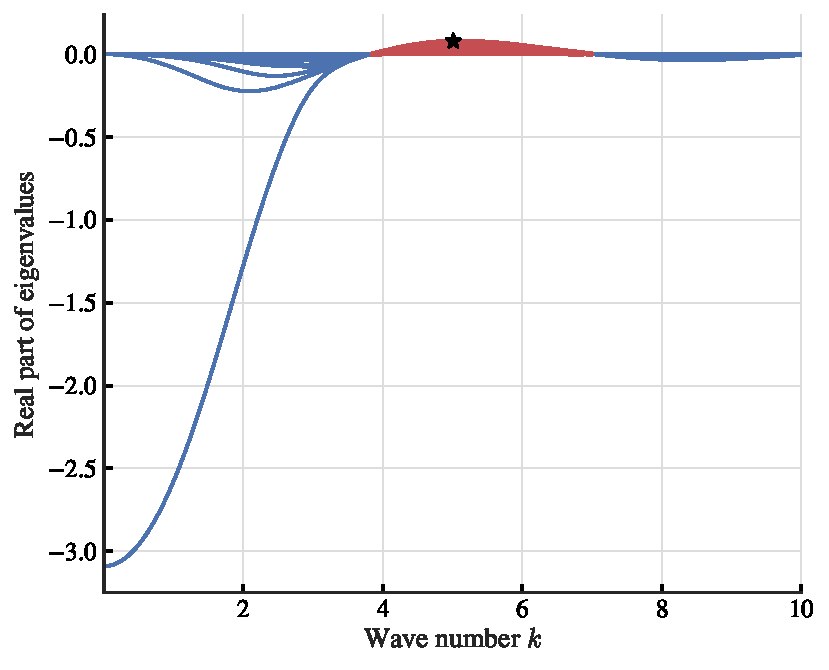
\includegraphics[width=0.6\textwidth]{./figs/continuous_spectrum.pdf}
    \caption{
        Continuous spectrum $\mathrm{Re}[ \lambda _{m}^{\left[ 0 \right]}\left( k \right) ]$ as a function of wave number $k$ for $K=20, d_0=1$.
    }
\end{figure}

% \begin{figure}[H]
%     \centering
%     \subcaptionbox{
%         $\mathrm{Re}[ \lambda _{m}^{\left[ 0 \right]}\left( k \right) ]$.
%         Different K have the same zero point.
%     }[0.49\linewidth]{
%         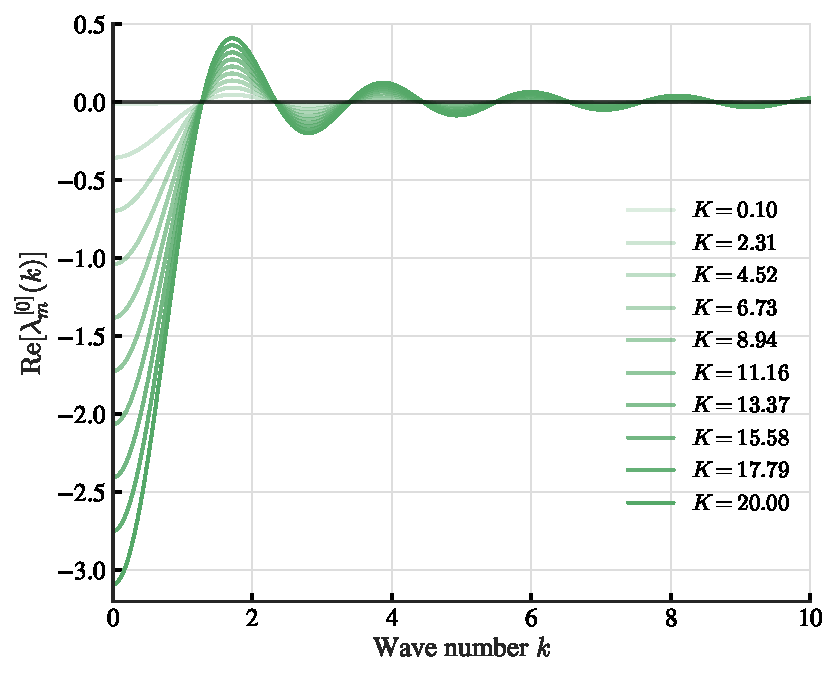
\includegraphics[width=\linewidth]{figs/phaseLagPatternFormation_lambda_m_varyK.pdf}
%     }
%     \hfill
%     \subcaptionbox{
%         The zero point of $\mathrm{Re}[ \lambda _{m}^{\left[ 0 \right]}\left( k \right) ]$ as a function of wave number $k$. The zero point solutions exhibit periodicity.
%     }[0.49\linewidth]{
%         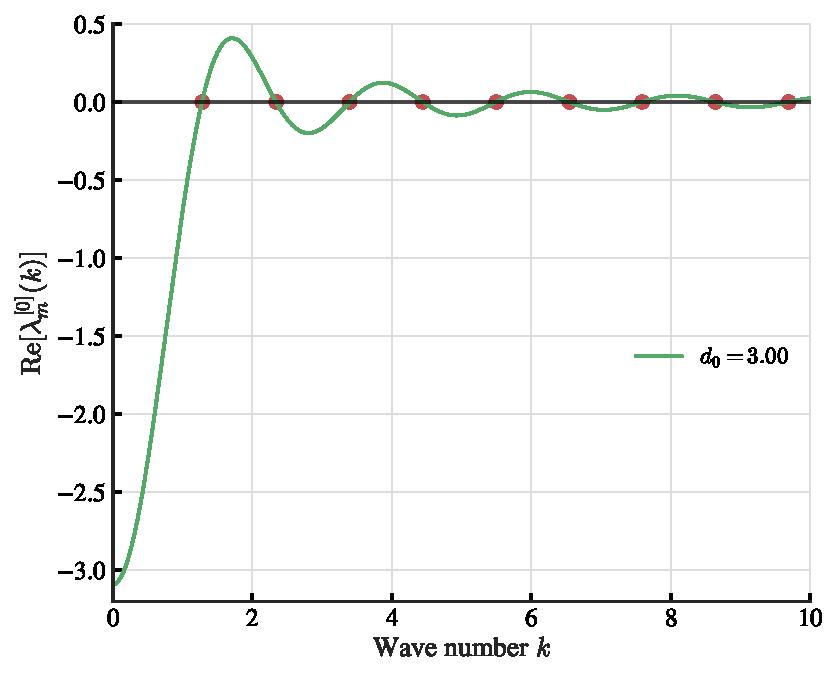
\includegraphics[width=\linewidth]{figs/phaseLagPatternFormation_lambda_m_zeroPoint.pdf}
%     }
%     \caption{
%         Simulation results for the linear stability analysis with $K=20$ and $\alpha=0.6\pi$.
%     }
% \end{figure}

% \begin{figure}[H]
%     \centering
%     \subcaptionbox{
%         $\mathrm{Re}[ \lambda _{m}^{\left[ 0 \right]}\left( k \right) ]$.
%         The smaller $d_0$, the slower the instability speed, which corresponding to the simulation.
%     }[0.49\linewidth]{
%         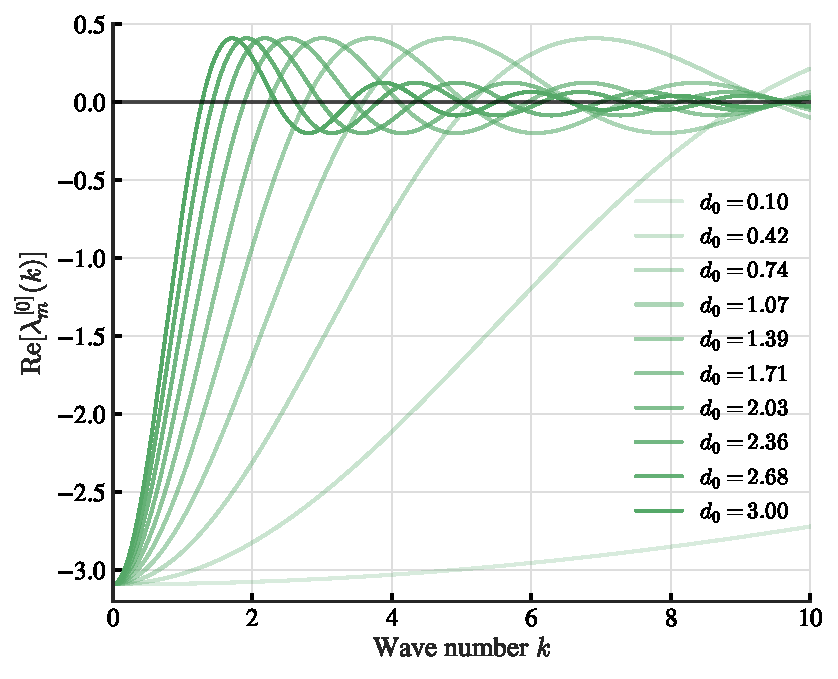
\includegraphics[width=\linewidth]{figs/phaseLagPatternFormation_lambda_m.pdf}
%     }
%     \hfill
%     \subcaptionbox{
%         Phase diagram of critical wave number $k^*$ (first zero point of $\mathrm{Re}[ \lambda _{m}^{\left[ 0 \right]}\left( k \right) ]$) as a function of $(K, d_0)$, 
%     }[0.49\linewidth]{
%         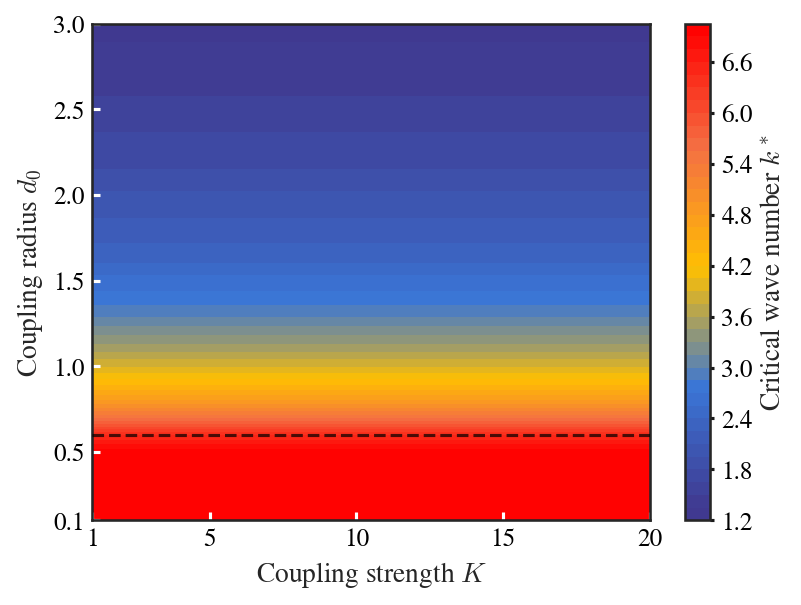
\includegraphics[width=\linewidth]{figs/orderParameter_Kstar_varying_strengthK_and_distanceD0.png}
%     }
%     \caption{
%         Simulation results for the linear stability analysis with $K=20$ and $\alpha=0.6\pi$.
%     }
% \end{figure}


\subsection{Abstract phase oscillator model}
Let us consider a decoupled phase-oscillator system 
\begin{equation}
    \dot{\theta}_i=\omega _i-K\sin \alpha +\frac{K}{N}\sum_{j=1}^N{\sin \left( \theta _j-\theta _i+\alpha \right)}\;.
    \label{eq:decoupledPhaseModel}
\end{equation}

To quantify the phase coherence of the system, it is convenient to define the generalized complex-valued order parameters, i.e.,
\begin{equation}
    \label{eq:orderParameter}
    Z\left( t \right) =R\left( t \right) \text{e}^{\text{i}\psi\left( t \right)}=\frac{1}{N}\sum_{j=1}^N{\text{e}^{\text{i}\theta _{j}\left( t \right)}}\;,
\end{equation}
where $n=1,2,\dots, N$, and $r\left( t \right)$, $\psi \left( t \right)$ are the amplitudes and arguments of the order parameter.
Our starting point is to analyze the critical point for the coherence of the order parameter.
In the thermodynamic limit $N\to \infty$, the state of the system in Eq.~(\ref{eq:decoupledPhaseModel}) can be characterized by the single-oscillator distribution $\rho\left( \theta ,\omega, t \right)$, which satisfies the continuity equation
\begin{equation}
    \frac{\partial \rho}{\partial t}+\frac{\partial \left( \rho v \right)}{\partial \theta}=0\;,
    \label{eq:continuityEquation}
\end{equation}
where $\rho \left( \theta ,\omega ,t \right)$ accounts for the fraction of oscillators with phase $\theta$ lying in the interval $\left( \theta ,\theta +\mathrm{d}\theta \right)$ at fixed frequency $\omega$ and time $t$, it satisfies the normalization condition
\begin{equation}
    \label{eq:normalization}
    \int_{0}^{2\pi}{\rho \left( \theta ,\omega ,t \right) \text{d}\theta} =1\;.
\end{equation}
Here, $v\left( \theta ,\omega ,t \right)$ is the velocity field, given by
\begin{equation}
    \begin{aligned}
        v\left( \theta ,\omega ,t \right) =&K\int_{-\infty}^{+\infty}{\int_0^{2\pi}{\sin \left( \theta ^{\prime}-\theta +\alpha \right) \rho \mathrm{d}\theta ^{\prime}\mathrm{d}\omega ^{\prime}}}\\
        &+\omega -K\sin \alpha \;.
    \end{aligned} 
\end{equation}
Correspondingly, the order parameter defined in Eq.~(\ref{eq:orderParameter}) in the thermodynamic limit reads
\begin{equation}
    Z\left( t \right) =\int_{-\infty}^{+\infty}{g\left(\omega\right)\mathrm{d}\omega \int_0^{2\pi}{\mathrm{e}^{\mathrm{i}\theta}\rho \left( \theta ,\omega ,t \right) \mathrm{d}\theta }} \;,
    \label{eq:orderParameterContinuum}
\end{equation}
then $v\left( \theta ,\omega ,t \right)$ simplifies to
\begin{equation}
    v\left( \theta ,\omega ,t \right) =\omega -K\sin \alpha +\mathrm{Im}\left[ H\left( t \right) \mathrm{e}^{-\mathrm{i}\theta} \right] \;,
    \label{eq:velocityField}
\end{equation}
with the mean-field being
\begin{equation}
    H\left( t \right) =KZ\left( t \right) \mathrm{e}^{\mathrm{i}\alpha} \;.
\end{equation}

Since the distribution $\rho \left( \theta ,\omega ,t \right)$ is $2\pi$-periodic in $\theta$, we can expand it in Fourier series as
\begin{equation}
    \rho \left( \theta ,\omega ,t \right) =\frac{1}{2\pi}\sum_{n=-\infty}^{+\infty}{a _n\left( \omega ,t \right) \mathrm{e}^{\mathrm{i}n\theta}}\;,
    \label{eq:rhoFourier}
\end{equation}
where $a _n\left( \omega ,t \right)$ is the $n$-th Fourier coefficient. In particular, we have $a _0\left( \omega ,t \right) \equiv 1$ owing to the normalization condition in Eq.~(\ref{eq:normalization}) and $a _{-n}\left( \omega ,t \right) =a _n^{*}\left( \omega ,t \right)$, where $*$ denotes the complex conjugate.

According to the Ott-Antonsen ansatz \cite{10.1063/1.2930766,10.1063/1.3136851}, it states that the $n$-th Fourier coefficient $a_n\left(\omega, t\right)$ can be expressed in terms of the first-order coefficient, i.e., $a_n\left(\omega, t\right) = a^{n}\left(\omega, t\right)$. In this regard, the evolution of $\rho\left(\theta, \omega, t\right)$ degenerates to an invariant manifold, which is
\begin{equation}
    \dot{a}\left( t \right) =\mathrm{i}\left( K\sin \alpha -\omega \right) a\left( t \right) +\frac{1}{2}\left[ H^{*}\left( t \right) -H\left( t \right) a^2\left( t \right) \right] \;.
    \label{eq:OttAntonsen}
\end{equation}
Consequently, Eq.~(\ref{eq:OttAntonsen}) is closed by the definition of the order parameter in Eq.~(\ref{eq:orderParameterContinuum}), where
\begin{equation}
    \begin{aligned}
        Z\left( t \right) &=\int_{-\infty}^{+\infty}{g\left( \omega \right) a_{-1}\left( \omega ,t \right) \mathrm{d}\omega} \;,\\
        &=\int_{-\infty}^{+\infty}{g\left( \omega \right) a^{*}\left( \omega ,t \right) \mathrm{d}\omega} \;.\\
    \end{aligned}
    \label{eq:orderParameterOttAntonsen}
\end{equation}

We stress that Eq.~(\ref{eq:OttAntonsen}) is still infinite dimensional
because of the distributed natural frequencies. Thus, we may make a specific choice for the frequency distribution to get around this difficulty, e.g. a Lorentzian distribution $g\left(\omega\right)=\varDelta / [ \pi\left(\omega-\mu\right)^2+\varDelta ^2 ]$ with $\varDelta $ being the width of the distribution and $\mu$ being the mean frequency.
In this setting, the order parameters defined in Eq.~(\ref{eq:orderParameterOttAntonsen}) can be calculated by using Cauchy's residue theorem with analytical continuation of $a\left(\omega, t\right)$ into the lower half complex plane, which leads to
\begin{equation}
    Z(t)=a^{*}\left(\mu-\mathrm{i}\varDelta, t\right) \;.
\end{equation}
As a result, the low-dimensional evolution of the order parameter can be obtained by replacing $\omega$ with $\mu-\mathrm{i}\varDelta$ and by taking into account the complex conjugate, which reads
\begin{equation}
    \dot{Z}=-\Delta Z+\mathrm{i}Z\left( \mu -K\sin \alpha \right) +\frac{1}{2}\left[ KZ\mathrm{e}^{\mathrm{i}\alpha}-KZ^*Z^2\mathrm{e}^{-\mathrm{i}\alpha} \right] \;.
    \label{eq:orderParameterEvolution}
\end{equation}
Rewrite above equation using polar coordinates $Z\left( t \right) =R\left( t \right) \mathrm{e}^{\mathrm{i}\psi \left( t \right)}$, we have
\begin{subequations}
    \begin{align}
        \dot{R}&=\frac{R}{2}\left( K-2\varDelta -KR^2 \right) \cos \alpha \;, \label{eq:dotAmplitudeR}\\
        \dot{\psi}&=\mu +\frac{K}{2}\left( R^2-1 \right) \sin \alpha \label{detPsi}\;.
    \end{align}
\end{subequations}
Obviously, the amplitude $R\left( t \right)$ is decoupled from the mean phase $\psi\left( t \right)$ and Eq.~(\ref{eq:dotAmplitudeR}) have a critical coupling strength $K_c=2\varDelta$ and a pair of critical phase frustration $\left|\alpha_c\right| = \pi/2$.
Let us first consider the simplest case of $ \varDelta =0, \mu=0$, which corresponds to the case of achiral particles. In this case, when $\left|\alpha_c\right| > \pi/2$, the system bifurcates to $R=0$, which corresponds to the incoherent state in phase oscillators and lattice state in self-propelled particles, while for $\left|\alpha_c\right| < \pi/2$, the system has a unique stable fixed point at $R=1$, which corresponds to the coherent state and swarming state, respectively.

For the incoherent state, the system is totally disordered with the phases distributed uniformly around the unit circle, i.e., $\rho\left(\theta, \omega, t\right) = g(\omega)/2\pi$, which implies that the phase velocity of each oscillator/particle becomes
\begin{equation}
    \dot{\theta}_i=\omega_i-K\sin \alpha \;.
\end{equation}
Correspondingly, the rotational radii of $i$-th particle is
\begin{equation}
    r_i=\frac{v}{\dot{\theta}_i}=\frac{v}{\omega _i-K\sin \alpha}\;.
\end{equation}

% $$
% \begin{aligned}
% \begin{aligned}
% 	\dot{\mathbf{r}}_i&=v\mathbf{p}\left( \theta _i \right)\\
% 	\dot{\theta}_i&=\omega _i+\frac{K}{\left| A_i \right|}\sum_{j\in A_i}{\left[ \sin \left( \theta _j-\theta _i+\alpha \right) -\sin \alpha \right]}\\
% \end{aligned}
% \\
% A_i=\left\{ j\mid \left| \mathbf{r}_i-\mathbf{r}_i \right|\leqslant d_0 \right\} 
% \\
% \frac{\partial \rho}{\partial t}=-v\mathbf{p}\left( \theta \right) \cdot \nabla \rho -\frac{\partial}{\partial \theta}\left\{ \mathcal{T} \left[ \rho \right] \rho \right\} 
% \\
% \mathcal{T} \left[ \rho \right] =\frac{K}{A}\int_{L\times L}{\mathrm{d}^2\mathbf{r}^{\prime}\int_0^{2\pi}{\mathrm{d}\theta ^{\prime}\rho \left( \mathbf{r}^{\prime},\theta ^{\prime},t \right) \Theta \left( \left| \mathbf{r}^{\prime}-\mathbf{r} \right|-d_0 \right) \left[ \sin \left( \theta ^{\prime}-\theta +\alpha \right) -\sin \alpha \right]}}
% \\
% A=\int_{L\times L}{\mathrm{d}^2\mathbf{r}^{\prime}\int_0^{2\pi}{\mathrm{d}\theta ^{\prime}\rho \left( \mathbf{r}^{\prime},\theta ^{\prime},t \right) \Theta \left( \left| \mathbf{r}^{\prime}-\mathbf{r} \right|-d_0 \right)}}
% \\
% \mathrm{For} \mathrm{all} \mathrm{to} \mathrm{all}
% \\
% p\left( \theta ,t \right) =\int_{L\times L}{\mathrm{d}^2\mathbf{r}\rho \left( \mathbf{r},\theta ,t \right)}
% \\
% \frac{\partial p}{\partial t}=-\frac{\partial}{\partial \theta}\left\{ \mathcal{T} \left[ \rho \right] \rho \right\} 
% \\
% \mathcal{T} \left[ \rho \right] =K\int_0^{2\pi}{\mathrm{d}\theta ^{\prime}p\left( \theta ^{\prime},t \right) \left[ \sin \left( \theta ^{\prime}-\theta +\alpha \right) -\sin \alpha \right]}
% \\
% p_0=\frac{1}{2\pi}
% \\
% p\left( \theta ,t \right) =p_0+\varepsilon \mathrm{e}^{\lambda t}\Phi \left( \theta \right) 
% \\
% \begin{aligned}
% 	\mathcal{T} \left[ \rho \right] &=K\int_0^{2\pi}{\mathrm{d}\theta ^{\prime}\left( p_0+\varepsilon \mathrm{e}^{\lambda t}\Phi \left( \theta ^{\prime} \right) \right) \left[ \sin \left( \theta ^{\prime}-\theta +\alpha \right) -\sin \alpha \right]}\\
% 	&=K\varepsilon \mathrm{e}^{\lambda t}\int_0^{2\pi}{\mathrm{d}\theta ^{\prime}\Phi \left( \theta ^{\prime} \right) \left[ \sin \left( \theta ^{\prime}-\theta +\alpha \right) -\sin \alpha \right]}\\
% \end{aligned}
% \\
% \mathcal{T} \left[ \rho \right] \rho \approx \frac{K\varepsilon \mathrm{e}^{\lambda t}}{2\pi}\int_0^{2\pi}{\mathrm{d}\theta ^{\prime}\Phi \left( \theta ^{\prime} \right) \left[ \sin \left( \theta ^{\prime}-\theta +\alpha \right) -\sin \alpha \right]}
% \\
% \frac{\partial}{\partial \theta}\left\{ \mathcal{T} \left[ \rho \right] \rho \right\} \approx \frac{\partial}{\partial \theta}\left\{ \frac{K\varepsilon \mathrm{e}^{\lambda t}}{2\pi}\int_0^{2\pi}{\mathrm{d}\theta ^{\prime}\Phi \left( \theta ^{\prime} \right) \left[ \sin \left( \theta ^{\prime}-\theta +\alpha \right) -\sin \alpha \right]} \right\} 
% \\
% \sin \left( \theta ^{\prime}-\theta +\alpha \right) =\sin \left( \theta ^{\prime}-\theta \right) \cos \alpha +\sin \alpha \cos \left( \theta ^{\prime}-\theta +\alpha \right) 
% \\
% \begin{aligned}
% 	\lambda \varepsilon \mathrm{e}^{\lambda t}\Phi \left( \theta \right) &=-\frac{\partial}{\partial \theta}\left\{ \frac{K\varepsilon \mathrm{e}^{\lambda t}}{2\pi}\int_0^{2\pi}{\mathrm{d}\theta ^{\prime}\Phi \left( \theta ^{\prime} \right) \left[ \sin \left( \theta ^{\prime}-\theta +\alpha \right) -\sin \alpha \right]} \right\}\\
% 	\lambda \Phi \left( \theta \right) &=-\frac{\partial}{\partial \theta}\left\{ \frac{K}{2\pi}\int_0^{2\pi}{\mathrm{d}\theta ^{\prime}\Phi \left( \theta ^{\prime} \right) \left[ \sin \left( \theta ^{\prime}-\theta +\alpha \right) -\sin \alpha \right]} \right\}\\
% \end{aligned}
% \\
% \mathcal{L} _{00}\Phi \left( \theta \right) =-\frac{\partial}{\partial \theta}\left\{ \frac{K}{2\pi}\int_0^{2\pi}{\mathrm{d}\theta ^{\prime}\Phi \left( \theta ^{\prime} \right) \left[ \sin \left( \theta ^{\prime}-\theta +\alpha \right) -\sin \alpha \right]} \right\} 
% \\
% \mathcal{L} _{00}\Phi =\lambda \Phi 
% \\
% \Phi \left( \theta \right) =\sum_{m=-\infty}^{+\infty}{c_m\mathrm{e}^{\mathrm{i}m\theta}}=\sum_{m=-\infty}^{+\infty}{c_m\Phi _m\left( \theta \right)}, \Phi _m\left( \theta \right) =\mathrm{e}^{\mathrm{i}m\theta}
% \\
% \begin{aligned}
% 	\int_0^{2\pi}{\mathrm{d}\theta ^{\prime}\Phi \left( \theta ^{\prime} \right) \left[ \sin \left( \theta ^{\prime}-\theta +\alpha \right) -\sin \alpha \right]}&=\int_0^{2\pi}{\mathrm{d}\theta ^{\prime}\sum_{m=-\infty}^{+\infty}{c_m\mathrm{e}^{\mathrm{i}m\theta ^{\prime}}}\left[ \sin \left( \theta ^{\prime}-\theta +\alpha \right) -\sin \alpha \right]}\\
% 	&=\sum_{m=-\infty}^{+\infty}{c_m\int_0^{2\pi}{\mathrm{d}\theta ^{\prime}\mathrm{e}^{\mathrm{i}m\theta ^{\prime}}\left[ \sin \left( \theta ^{\prime}-\theta +\alpha \right) -\sin \alpha \right]}}\\
% \end{aligned}
% \\
% \begin{aligned}
% 	\int_0^{2\pi}{\mathrm{d}\theta ^{\prime}\mathrm{e}^{\mathrm{i}m\theta ^{\prime}}\left[ \sin \left( \theta ^{\prime}-\theta +\alpha \right) -\sin \alpha \right]}&=\int_0^{2\pi}{\mathrm{d}\theta ^{\prime}\mathrm{e}^{\mathrm{i}m\theta ^{\prime}}\sin \left( \theta ^{\prime}-\theta +\alpha \right)}-\sin \alpha \int_0^{2\pi}{\mathrm{d}\theta ^{\prime}\mathrm{e}^{\mathrm{i}m\theta ^{\prime}}}\\
% 	&=-2\pi \delta _{m,0}\sin \alpha +\frac{1}{2\mathrm{i}}\int_0^{2\pi}{\mathrm{d}\theta ^{\prime}\mathrm{e}^{\mathrm{i}m\theta ^{\prime}}\left[ \mathrm{e}^{\mathrm{i}\left( \theta ^{\prime}-\theta +\alpha \right)}-\mathrm{e}^{-\mathrm{i}\left( \theta ^{\prime}-\theta +\alpha \right)} \right]}\\
% 	&=-2\pi \delta _{m,0}\sin \alpha +\frac{\mathrm{e}^{-\mathrm{i}\left( \theta -\alpha \right)}}{2\mathrm{i}}\int_0^{2\pi}{\mathrm{d}\theta ^{\prime}\mathrm{e}^{\mathrm{i}\left( m+1 \right) \theta ^{\prime}}}-\frac{\mathrm{e}^{\mathrm{i}\left( \theta -\alpha \right)}}{2\mathrm{i}}\int_0^{2\pi}{\mathrm{d}\theta ^{\prime}\mathrm{e}^{\mathrm{i}\left( m-1 \right) \theta ^{\prime}}}\\
% 	&=-2\pi \delta _{m,0}\sin \alpha -\mathrm{i}\pi \delta _{m,-1}\mathrm{e}^{-\mathrm{i}\left( \theta -\alpha \right)}+\mathrm{i}\pi \delta _{m,1}\mathrm{e}^{\mathrm{i}\left( \theta -\alpha \right)}\\
% \end{aligned}
% \\
% \frac{\partial}{\partial \theta}\left\{ \frac{K}{2\pi}\int_0^{2\pi}{\mathrm{d}\theta ^{\prime}\mathrm{e}^{\mathrm{i}m\theta ^{\prime}}\left[ \sin \left( \theta ^{\prime}-\theta +\alpha \right) -\sin \alpha \right]} \right\} =-\frac{K\delta _{m,-1}}{2}\mathrm{e}^{-\mathrm{i}\left( \theta -\alpha \right)}-\frac{K\delta _{m,1}}{2}\mathrm{e}^{\mathrm{i}\left( \theta -\alpha \right)}
% \\
% \begin{aligned}
% 	\mathcal{L} _{00}\sum_{m=-\infty}^{+\infty}{c_m\mathrm{e}^{\mathrm{i}m\theta}}&=\lambda \sum_{m=-\infty}^{+\infty}{c_m\mathrm{e}^{\mathrm{i}m\theta}}\\
% 	\mathcal{L} _{00}\mathrm{e}^{\mathrm{i}m\theta}&=\lambda _m\mathrm{e}^{\mathrm{i}m\theta}\\
% 	\lambda _m\mathrm{e}^{\mathrm{i}m\theta}&=-\frac{\partial}{\partial \theta}\left\{ \frac{K}{2\pi}\int_0^{2\pi}{\mathrm{d}\theta ^{\prime}\mathrm{e}^{\mathrm{i}m\theta}\left[ \sin \left( \theta ^{\prime}-\theta +\alpha \right) -\sin \alpha \right]} \right\}\\
% 	\lambda _m\mathrm{e}^{\mathrm{i}m\theta}&=\frac{K\delta _{m,-1}}{2}\mathrm{e}^{-\mathrm{i}\left( \theta -\alpha \right)}+\frac{K\delta _{m,1}}{2}\mathrm{e}^{\mathrm{i}\left( \theta -\alpha \right)}\\
% 	\lambda _m&=\frac{K}{2}\left( \delta _{m,-1}\mathrm{e}^{\mathrm{i}\alpha}+\delta _{m,1}\mathrm{e}^{-\mathrm{i}\alpha} \right)\\
% \end{aligned}
% \\
% \mathrm{For} \mathrm{finite} \mathrm{range}
% \\
% \rho _0=\frac{1}{2\pi L^2}
% \\
% \rho \left( \mathbf{r},\theta ,t \right) =\rho _0+\varepsilon \mathrm{e}^{\lambda \left( k \right) t+\mathrm{i}\mathbf{k}\cdot \mathbf{r}}\Phi \left( \theta \right) , k=\left| \mathbf{k} \right|
% \\
% \frac{\partial \rho}{\partial t}=\varepsilon \lambda \mathrm{e}^{\lambda \left( k \right) t+\mathrm{i}\mathbf{k}\cdot \mathbf{r}}\Phi \left( \theta \right) 
% \\
% -v\mathbf{p}\left( \theta \right) \cdot \nabla \rho =-v\mathbf{p}\left( \theta \right) \cdot \left[ \mathrm{i}\mathbf{k}\varepsilon \mathrm{e}^{\lambda t+\mathrm{i}\mathbf{k}\cdot \mathbf{r}}\Phi \left( \theta \right) \right] =-\mathrm{i}v\varepsilon \mathrm{e}^{\lambda t+\mathrm{i}\mathbf{k}\cdot \mathbf{r}}\Phi \left( \theta \right) \mathbf{p}\left( \theta \right) \cdot \mathbf{k}
% \\
% \Theta _k=\int{\mathrm{d}^2\mathbf{R}\Theta \left( \left| \mathbf{R} \right|-d_0 \right) \mathrm{e}^{\mathrm{i}\mathbf{k}\cdot \mathbf{R}}}
% \\
% \begin{aligned}
% 	A&=\int_{L\times L}{\mathrm{d}^2\mathbf{r}^{\prime}\int_0^{2\pi}{\mathrm{d}\theta ^{\prime}\rho \left( \mathbf{r}^{\prime},\theta ^{\prime},t \right) \Theta \left( \left| \mathbf{r}^{\prime}-\mathbf{r} \right|-d_0 \right)}}\\
% 	&=\int_{L\times L}{\mathrm{d}^2\mathbf{r}^{\prime}\int_0^{2\pi}{\mathrm{d}\theta ^{\prime}\left[ \rho _0+\varepsilon \mathrm{e}^{\lambda t+\mathrm{i}\mathbf{k}\cdot \mathbf{r}^{\prime}}\Phi \left( \theta ^{\prime} \right) \right] \Theta \left( \left| \mathbf{r}^{\prime}-\mathbf{r} \right|-d_0 \right)}}\\
% 	&=\frac{1}{L^2}\int_{L\times L}{\mathrm{d}^2\mathbf{r}^{\prime}\Theta \left( \left| \mathbf{r}^{\prime}-\mathbf{r} \right|-d_0 \right)}+\varepsilon \mathrm{e}^{\lambda t}\int_{L\times L}{\mathrm{d}^2\mathbf{r}^{\prime}\Theta \left( \left| \mathbf{r}^{\prime}-\mathbf{r} \right|-d_0 \right) \mathrm{e}^{\mathrm{i}\mathbf{k}\cdot \mathbf{r}^{\prime}}\int_0^{2\pi}{\mathrm{d}\theta ^{\prime}\Phi \left( \theta ^{\prime} \right)}}\\
% 	&=\frac{1}{L^2}\int_{L\times L}{\mathrm{d}^2\mathbf{R}\Theta \left( \left| \mathbf{R} \right|-d_0 \right)}+\varepsilon \mathrm{e}^{\lambda t+\mathrm{i}\mathbf{k}\cdot \mathbf{r}}\int_{L\times L}{\mathrm{d}^2\mathbf{R}\Theta \left( \left| \mathbf{R} \right|-d_0 \right) \mathrm{e}^{\mathrm{i}\mathbf{k}\cdot \mathbf{R}}\int_0^{2\pi}{\mathrm{d}\theta ^{\prime}\Phi \left( \theta ^{\prime} \right)}}\\
% 	&=\frac{1}{L^2}\Theta _0+\varepsilon \mathrm{e}^{\lambda t+\mathrm{i}\mathbf{k}\cdot \mathbf{r}}\Theta _k\int_0^{2\pi}{\mathrm{d}\theta ^{\prime}\Phi \left( \theta ^{\prime} \right)}\\
% \end{aligned}
% \\
% \begin{aligned}
% 	\mathcal{T} \left[ \rho \right] &=\frac{K}{A}\int_{L\times L}{\mathrm{d}^2\mathbf{r}^{\prime}\int_0^{2\pi}{\mathrm{d}\theta ^{\prime}\rho \left( \mathbf{r}^{\prime},\theta ^{\prime},t \right) \Theta \left( \left| \mathbf{r}^{\prime}-\mathbf{r} \right|-d_0 \right) \left[ \sin \left( \theta ^{\prime}-\theta +\alpha \right) -\sin \alpha \right]}}\\
% 	&=\frac{K}{A}\int_{L\times L}{\mathrm{d}^2\mathbf{r}^{\prime}\int_0^{2\pi}{\mathrm{d}\theta ^{\prime}\left[ \rho _0+\varepsilon \mathrm{e}^{\lambda t+\mathrm{i}\mathbf{k}\cdot \mathbf{r}^{\prime}}\Phi \left( \theta ^{\prime} \right) \right] \Theta \left( \left| \mathbf{r}^{\prime}-\mathbf{r} \right|-d_0 \right) \left[ \sin \left( \theta ^{\prime}-\theta +\alpha \right) -\sin \alpha \right]}}\\
% 	&=-\frac{K\sin \alpha}{L^2A}\int_{L\times L}{\mathrm{d}^2\mathbf{R}\Theta \left( \left| \mathbf{R} \right|-d_0 \right)}+\frac{K\varepsilon}{A}\mathrm{e}^{\lambda t+\mathrm{i}\mathbf{k}\cdot \mathbf{r}}\int_{L\times L}{\mathrm{d}^2\mathbf{R}\Theta \left( \left| \mathbf{R} \right|-d_0 \right) \mathrm{e}^{\mathrm{i}\mathbf{k}\cdot \mathbf{R}}\int_0^{2\pi}{\mathrm{d}\theta ^{\prime}\Phi \left( \theta ^{\prime} \right) \left[ \sin \left( \theta ^{\prime}-\theta +\alpha \right) -\sin \alpha \right]}}\\
% 	&=-\frac{K\sin \alpha}{L^2A}\Theta _0+\frac{K\varepsilon}{A}\mathrm{e}^{\lambda t+\mathrm{i}\mathbf{k}\cdot \mathbf{r}}\Theta _k\int_0^{2\pi}{\mathrm{d}\theta ^{\prime}\Phi \left( \theta ^{\prime} \right) \left[ \sin \left( \theta ^{\prime}-\theta +\alpha \right) -\sin \alpha \right]}\\
% 	&=\frac{K}{A}\left\{ -\frac{\Theta _0\sin \alpha}{L^2}+\varepsilon \mathrm{e}^{\lambda t+\mathrm{i}\mathbf{k}\cdot \mathbf{r}}\Theta _k\int_0^{2\pi}{\mathrm{d}\theta ^{\prime}\Phi \left( \theta ^{\prime} \right) \left[ \sin \left( \theta ^{\prime}-\theta +\alpha \right) -\sin \alpha \right]} \right\}\\
% \end{aligned}
% \\
% \mathcal{T} \left[ \rho \right] \rho \approx \frac{1}{2\pi L^2}\frac{K}{A}\left\{ -\frac{\Theta _0\sin \alpha}{L^2}+\varepsilon \mathrm{e}^{\lambda t+\mathrm{i}\mathbf{k}\cdot \mathbf{r}}\Theta _k\int_0^{2\pi}{\mathrm{d}\theta ^{\prime}\Phi \left( \theta ^{\prime} \right) \left[ \sin \left( \theta ^{\prime}-\theta +\alpha \right) -\sin \alpha \right]} \right\} 
% \\
% \frac{\partial}{\partial \theta}\left\{ \mathcal{T} \left[ \rho \right] \rho \right\} \approx \frac{1}{2\pi L^2}\frac{K}{A}\varepsilon \mathrm{e}^{\lambda t+\mathrm{i}\mathbf{k}\cdot \mathbf{r}}\Theta _k\frac{\partial}{\partial \theta}\left\{ \int_0^{2\pi}{\mathrm{d}\theta ^{\prime}\Phi \left( \theta ^{\prime} \right) \left[ \sin \left( \theta ^{\prime}-\theta +\alpha \right) -\sin \alpha \right]} \right\} 
% \\
% \begin{aligned}
% 	\frac{\partial \rho}{\partial t}&=-v\mathbf{p}\left( \theta \right) \cdot \nabla \rho -\frac{\partial}{\partial \theta}\left\{ \mathcal{T} \left[ \rho \right] \rho \right\}\\
% 	\varepsilon \lambda \mathrm{e}^{\lambda \left( k \right) t+\mathrm{i}\mathbf{k}\cdot \mathbf{r}}\Phi \left( \theta \right) &=-\mathrm{i}v\varepsilon \mathrm{e}^{\lambda t+\mathrm{i}\mathbf{k}\cdot \mathbf{r}}\left( \mathbf{p}\left( \theta \right) \cdot \mathbf{k} \right) \Phi \left( \theta \right) -\frac{1}{2\pi L^2}\frac{K}{A}\varepsilon \mathrm{e}^{\lambda t+\mathrm{i}\mathbf{k}\cdot \mathbf{r}}\Theta _k\frac{\partial}{\partial \theta}\left\{ \int_0^{2\pi}{\mathrm{d}\theta ^{\prime}\Phi \left( \theta ^{\prime} \right) \left[ \sin \left( \theta ^{\prime}-\theta +\alpha \right) -\sin \alpha \right]} \right\}\\
% 	\lambda \Phi \left( \theta \right) &=-\mathrm{i}v\left( \mathbf{p}\left( \theta \right) \cdot \mathbf{k} \right) \Phi \left( \theta \right) -\frac{K\Theta _k}{2\pi L^2A}\frac{\partial}{\partial \theta}\left\{ \int_0^{2\pi}{\mathrm{d}\theta ^{\prime}\Phi \left( \theta ^{\prime} \right) \left[ \sin \left( \theta ^{\prime}-\theta +\alpha \right) -\sin \alpha \right]} \right\}\\
% 	\mathcal{L} \Phi &=\left( \mathcal{L} _0-\mathrm{i}vk\mathcal{L} _1 \right) \Phi =\lambda \Phi\\
% \end{aligned}
% \\
% \begin{aligned}
% 	\mathcal{L} _0\Phi &=-\frac{K\Theta _k}{2\pi L^2A}\frac{\partial}{\partial \theta}\left\{ \int_0^{2\pi}{\mathrm{d}\theta ^{\prime}\Phi \left( \theta ^{\prime} \right) \left[ \sin \left( \theta ^{\prime}-\theta +\alpha \right) -\sin \alpha \right]} \right\}\\
% 	\mathcal{L} _1\Phi &=\left( \mathbf{p}\left( \theta \right) \cdot \bar{\mathbf{k}} \right) \Phi , \bar{\mathbf{k}}=\mathbf{k}/k\\
% \end{aligned}
% \\
% \Phi \left( \theta \right) =\sum_{m=-\infty}^{+\infty}{c_m\mathrm{e}^{\mathrm{i}m\theta}}=\sum_{m=-\infty}^{+\infty}{c_m\Phi _m\left( \theta \right)}, \Phi _m\left( \theta \right) =\mathrm{e}^{\mathrm{i}m\theta}
% \\
% \begin{array}{c}
% 	\mathcal{L} \sum_{m=-\infty}^{+\infty}{c_m\mathrm{e}^{\mathrm{i}m\theta}}=\lambda \sum_{m=-\infty}^{+\infty}{c_m\mathrm{e}^{\mathrm{i}m\theta}}\\
% 	\mathcal{L} \Phi _m=\lambda _m\Phi _m\\
% \end{array}
% \\
% \mathcal{L} _0\Phi _m=\lambda _{m}^{\left[ 0 \right]}\mathrm{e}^{\mathrm{i}m\theta}=-\frac{K\Theta _k}{2\pi L^2A_m}\frac{\partial}{\partial \theta}\left\{ \int_0^{2\pi}{\mathrm{d}\theta ^{\prime}\mathrm{e}^{\mathrm{i}m\theta}\left[ \sin \left( \theta ^{\prime}-\theta +\alpha \right) -\sin \alpha \right]} \right\} 
% \\
% A_m=\frac{1}{L^2}\Theta _0+\varepsilon \mathrm{e}^{\lambda t+\mathrm{i}\mathbf{k}\cdot \mathbf{r}}\Theta _k\int_0^{2\pi}{\mathrm{d}\theta ^{\prime}\mathrm{e}^{\mathrm{i}m\theta}}=\frac{1}{L^2}\Theta _0
% \\
% \mathcal{L} _1\Phi _m=\mathcal{L} _1\mathrm{e}^{\mathrm{i}m\theta}=\left( \mathbf{p}\left( \theta \right) \cdot \bar{\mathbf{k}} \right) \mathrm{e}^{\mathrm{i}m\theta}=\cos \theta \mathrm{e}^{\mathrm{i}m\theta}=\left( e^{i\left( m+1 \right) \theta}+e^{i\left( m-1 \right) \theta} \right) /2\;\left( \mathrm{Let} \mathbf{k}\,\,\mathrm{along} x-\mathrm{direction} \right) 
% \\
% \begin{aligned}
% 	\int_0^{2\pi}{\mathrm{d}\theta ^{\prime}\Phi \left( \theta ^{\prime} \right) \left[ \sin \left( \theta ^{\prime}-\theta +\alpha \right) -\sin \alpha \right]}&=\int_0^{2\pi}{\mathrm{d}\theta ^{\prime}\sum_{m=-\infty}^{+\infty}{c_m\mathrm{e}^{\mathrm{i}m\theta ^{\prime}}}\left[ \sin \left( \theta ^{\prime}-\theta +\alpha \right) -\sin \alpha \right]}\\
% 	&=\sum_{m=-\infty}^{+\infty}{c_m\int_0^{2\pi}{\mathrm{d}\theta ^{\prime}\mathrm{e}^{\mathrm{i}m\theta ^{\prime}}\left[ \sin \left( \theta ^{\prime}-\theta +\alpha \right) -\sin \alpha \right]}}\\
% \end{aligned}
% \\
% \begin{aligned}
% 	\int_0^{2\pi}{\mathrm{d}\theta ^{\prime}\mathrm{e}^{\mathrm{i}m\theta ^{\prime}}\left[ \sin \left( \theta ^{\prime}-\theta +\alpha \right) -\sin \alpha \right]}&=\int_0^{2\pi}{\mathrm{d}\theta ^{\prime}\mathrm{e}^{\mathrm{i}m\theta ^{\prime}}\sin \left( \theta ^{\prime}-\theta +\alpha \right)}-\sin \alpha \int_0^{2\pi}{\mathrm{d}\theta ^{\prime}\mathrm{e}^{\mathrm{i}m\theta ^{\prime}}}\\
% 	&=-2\pi \delta _{m,0}\sin \alpha +\frac{1}{2\mathrm{i}}\int_0^{2\pi}{\mathrm{d}\theta ^{\prime}\mathrm{e}^{\mathrm{i}m\theta ^{\prime}}\left[ \mathrm{e}^{\mathrm{i}\left( \theta ^{\prime}-\theta +\alpha \right)}-\mathrm{e}^{-\mathrm{i}\left( \theta ^{\prime}-\theta +\alpha \right)} \right]}\\
% 	&=-2\pi \delta _{m,0}\sin \alpha +\frac{\mathrm{e}^{-\mathrm{i}\left( \theta -\alpha \right)}}{2\mathrm{i}}\int_0^{2\pi}{\mathrm{d}\theta ^{\prime}\mathrm{e}^{\mathrm{i}\left( m+1 \right) \theta ^{\prime}}}-\frac{\mathrm{e}^{\mathrm{i}\left( \theta -\alpha \right)}}{2\mathrm{i}}\int_0^{2\pi}{\mathrm{d}\theta ^{\prime}\mathrm{e}^{\mathrm{i}\left( m-1 \right) \theta ^{\prime}}}\\
% 	&=-2\pi \delta _{m,0}\sin \alpha -\mathrm{i}\pi \delta _{m,-1}\mathrm{e}^{-\mathrm{i}\left( \theta -\alpha \right)}+\mathrm{i}\pi \delta _{m,1}\mathrm{e}^{\mathrm{i}\left( \theta -\alpha \right)}\\
% \end{aligned}
% \\
% \frac{\partial}{\partial \theta}\left\{ \int_0^{2\pi}{\mathrm{d}\theta ^{\prime}\mathrm{e}^{\mathrm{i}m\theta}\left[ \sin \left( \theta ^{\prime}-\theta +\alpha \right) -\sin \alpha \right]} \right\} =-\pi \delta _{m,-1}\mathrm{e}^{-\mathrm{i}\left( \theta -\alpha \right)}-\pi \delta _{m,1}\mathrm{e}^{\mathrm{i}\left( \theta -\alpha \right)}
% \\
% \begin{aligned}
% 	\lambda _{m}^{\left[ 0 \right]}\left( k \right) \mathrm{e}^{\mathrm{i}m\theta}&=\frac{K\Theta _k}{2\Theta _0}\left( \delta _{m,-1}\mathrm{e}^{-\mathrm{i}\left( \theta -\alpha \right)}+\delta _{m,1}\mathrm{e}^{\mathrm{i}\left( \theta -\alpha \right)} \right)\\
% 	\lambda _{m}^{\left[ 0 \right]}\left( k \right) &=\frac{K\Theta _k}{2\Theta _0}\left( \delta _{m,-1}\mathrm{e}^{\mathrm{i}\alpha}+\delta _{m,1}\mathrm{e}^{-\mathrm{i}\alpha} \right)\\
% \end{aligned}
% \\
% \Theta _k=\int{\mathrm{d}^2\mathbf{R}\Theta \left( \left| \mathbf{R} \right|-d_0 \right) \mathrm{e}^{\mathrm{i}\mathbf{k}\cdot \mathbf{R}}}
% \\
% \end{aligned}
% $$

\bibliography{ref}

\end{document}